%!TEX root = ../main.tex

\chapter{Potassium tracking analysis plots}%
\label{apdx:kmodelplots}

The results of the potassium tracking analysis of \gerdatwo\ data described in
\cref{sec:bkg:raw:ph2:kmodel} are reported here. The four series of plots that follow
represent the background decomposition of potassium events classified according to the
detectors in which an energy deposition was registered. Two models have been developed: a
base model and an extended model including pdfs for each separate detector string.  In
\cref{fig:bkg:raw:ph2:kmodel:base:results:M1,fig:bkg:raw:ph2:kmodel:base:results:M2} the
first two series of plots the results for single-detector and two-detector events in the
base model are given. The two last series in
\cref{fig:bkg:raw:ph2:kmodel:extended:results:M1,fig:bkg:raw:ph2:kmodel:extended:results:M2}
refer to the extended model.

Some components are merged together to improve the readability: in the \m{K40} plots
combined components are shown for \kvz\ and \Bih, while \kvn\ sources are grouped in close
(flat cables, holders, mini-shrouds) and far (fibers, SiPMs, copper shrouds, front-end
electronics) locations from the detector array. To visualize the two-detector data a
one-dimensional histogram has been obtained by summing together the projections on the two
domain axes (index $i$ and index $j$ in \cref{eq:bkg:raw:ph2:kmodel:likelihood}) of the
original two-dimensional histogram.

\begin{figure}
  \centering
  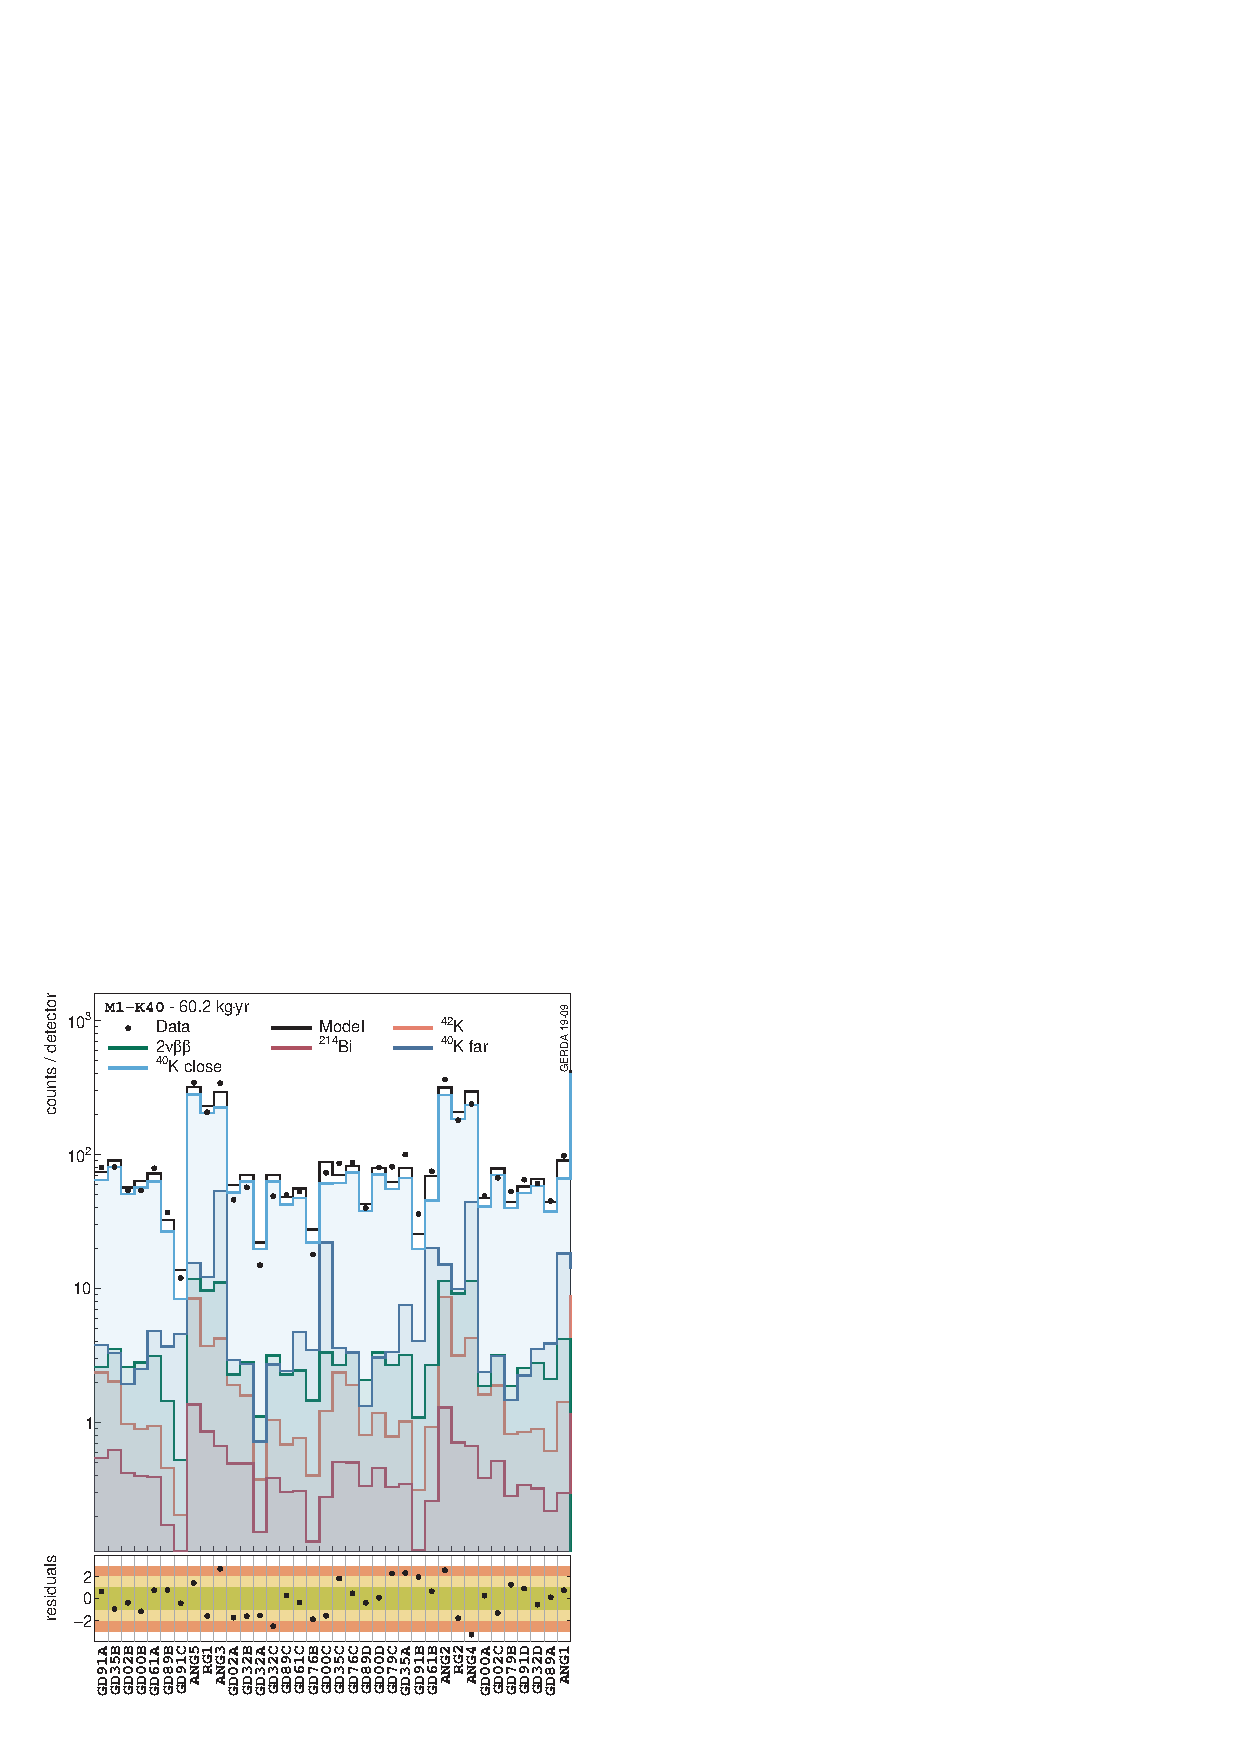
\includegraphics[width=0.45\textwidth]{plots/bkg/raw/ph2/results/kmodel/kmodel-1d-ds0.pdf}
  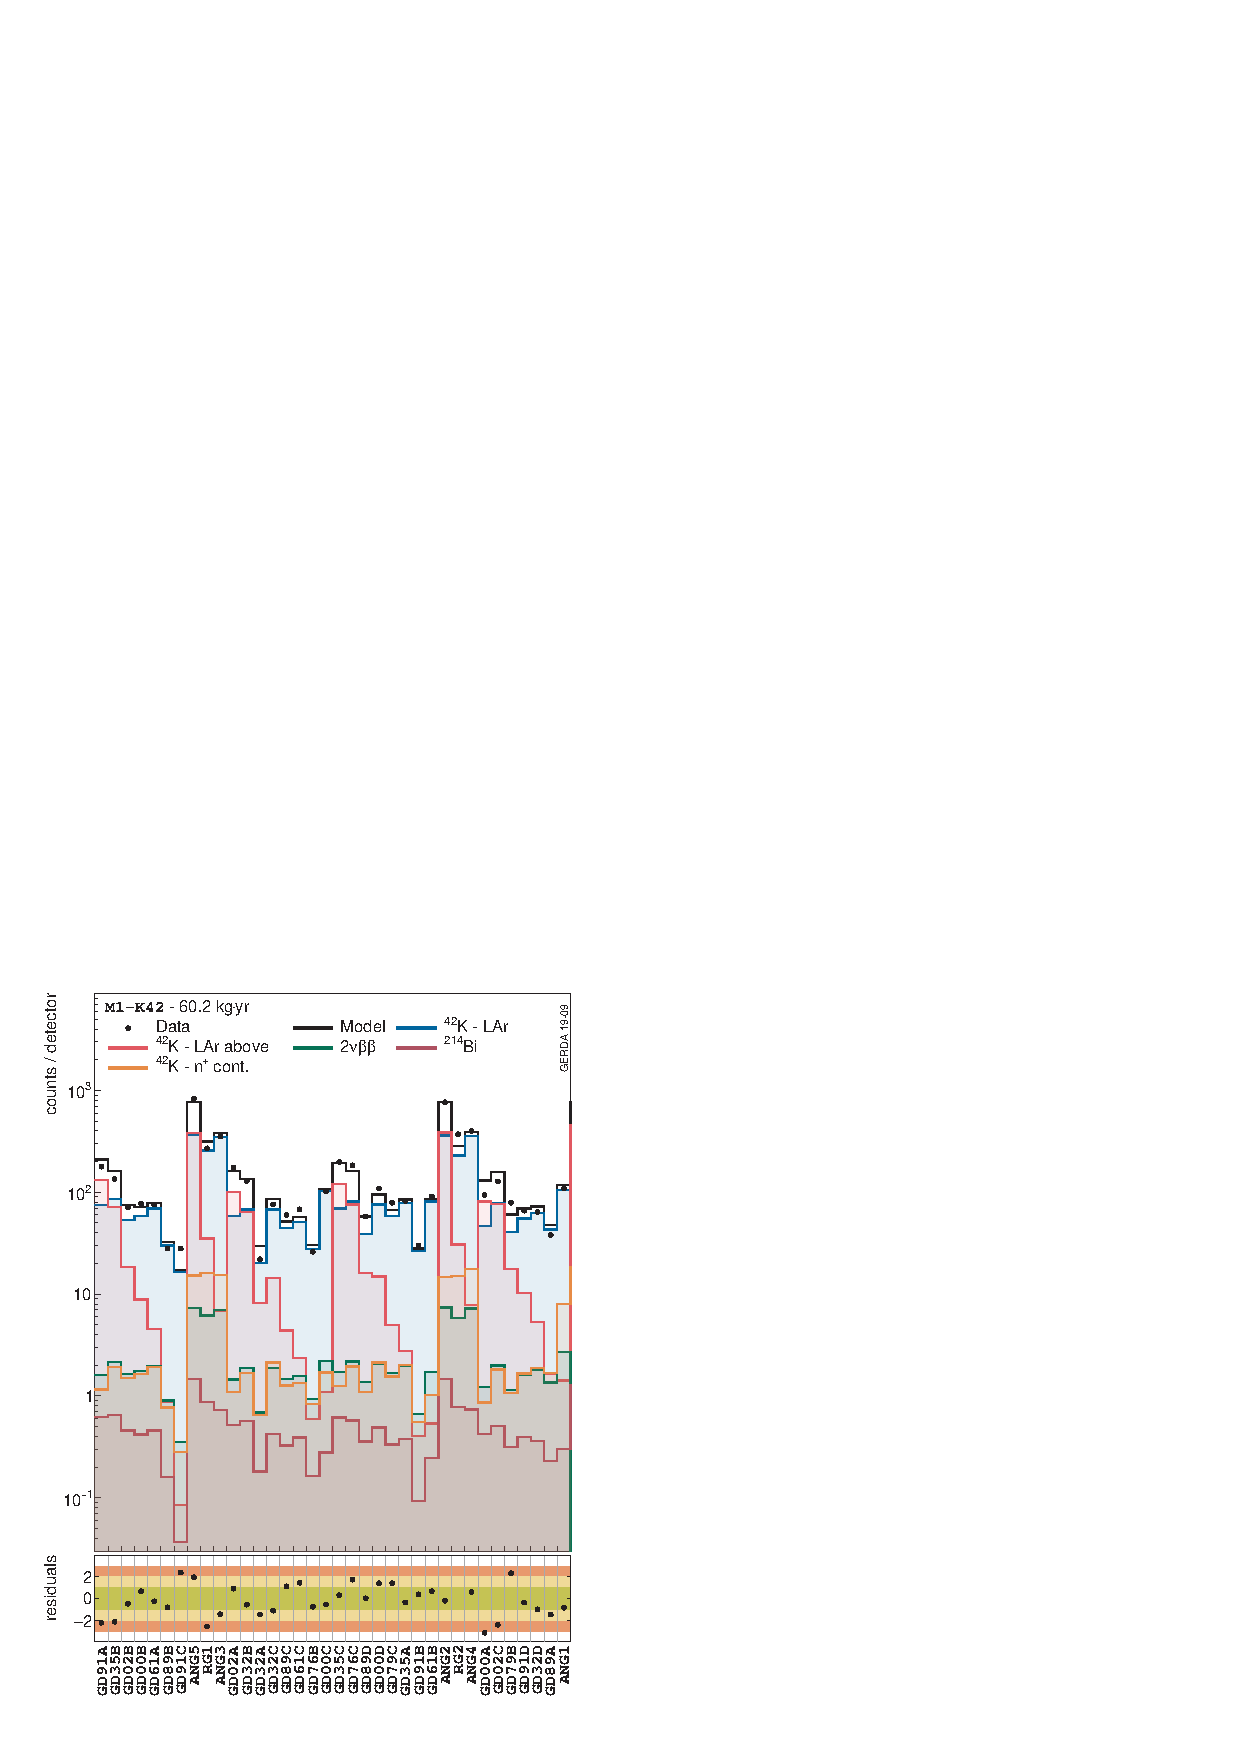
\includegraphics[width=0.45\textwidth]{plots/bkg/raw/ph2/results/kmodel/kmodel-1d-ds1.pdf}\vspace{10pt}
  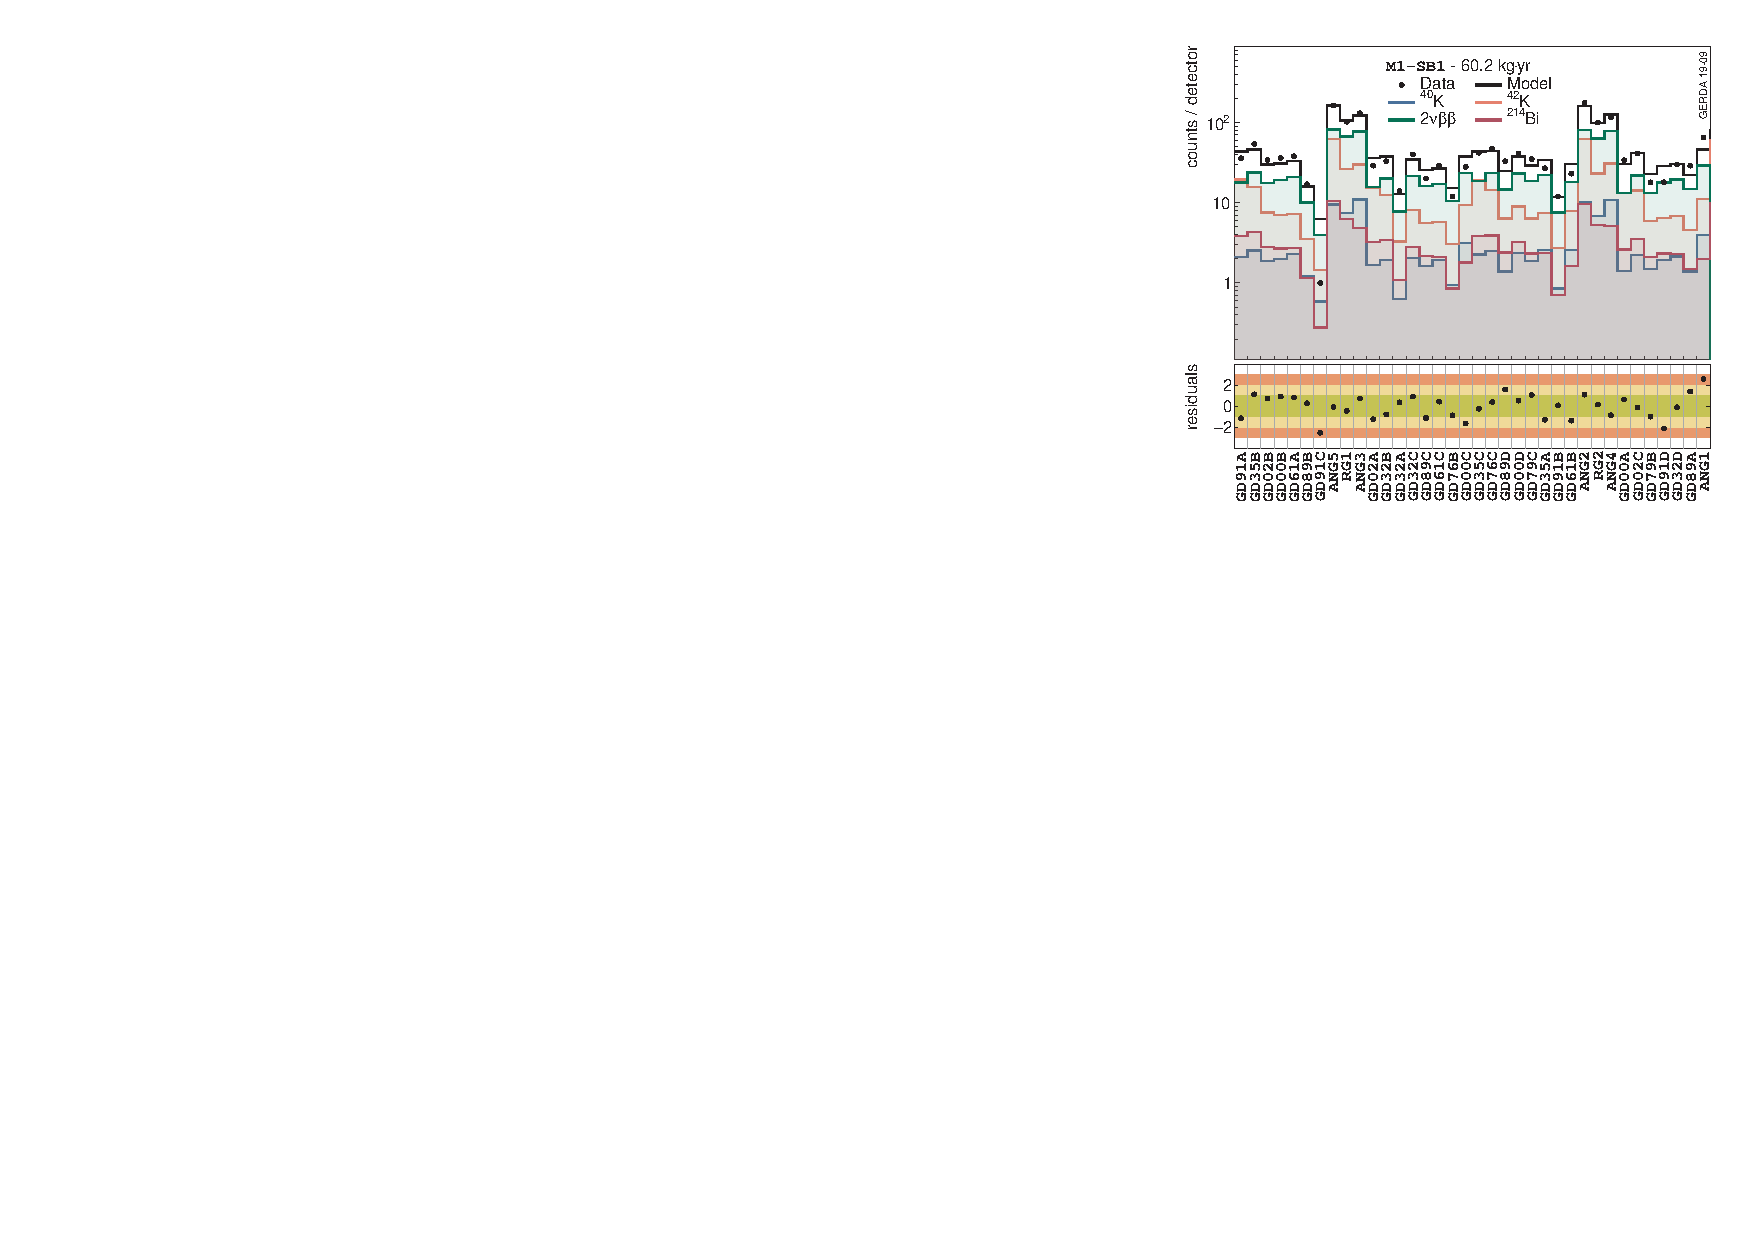
\includegraphics[width=0.45\textwidth]{plots/bkg/raw/ph2/results/kmodel/kmodel-1d-ds2.pdf}
  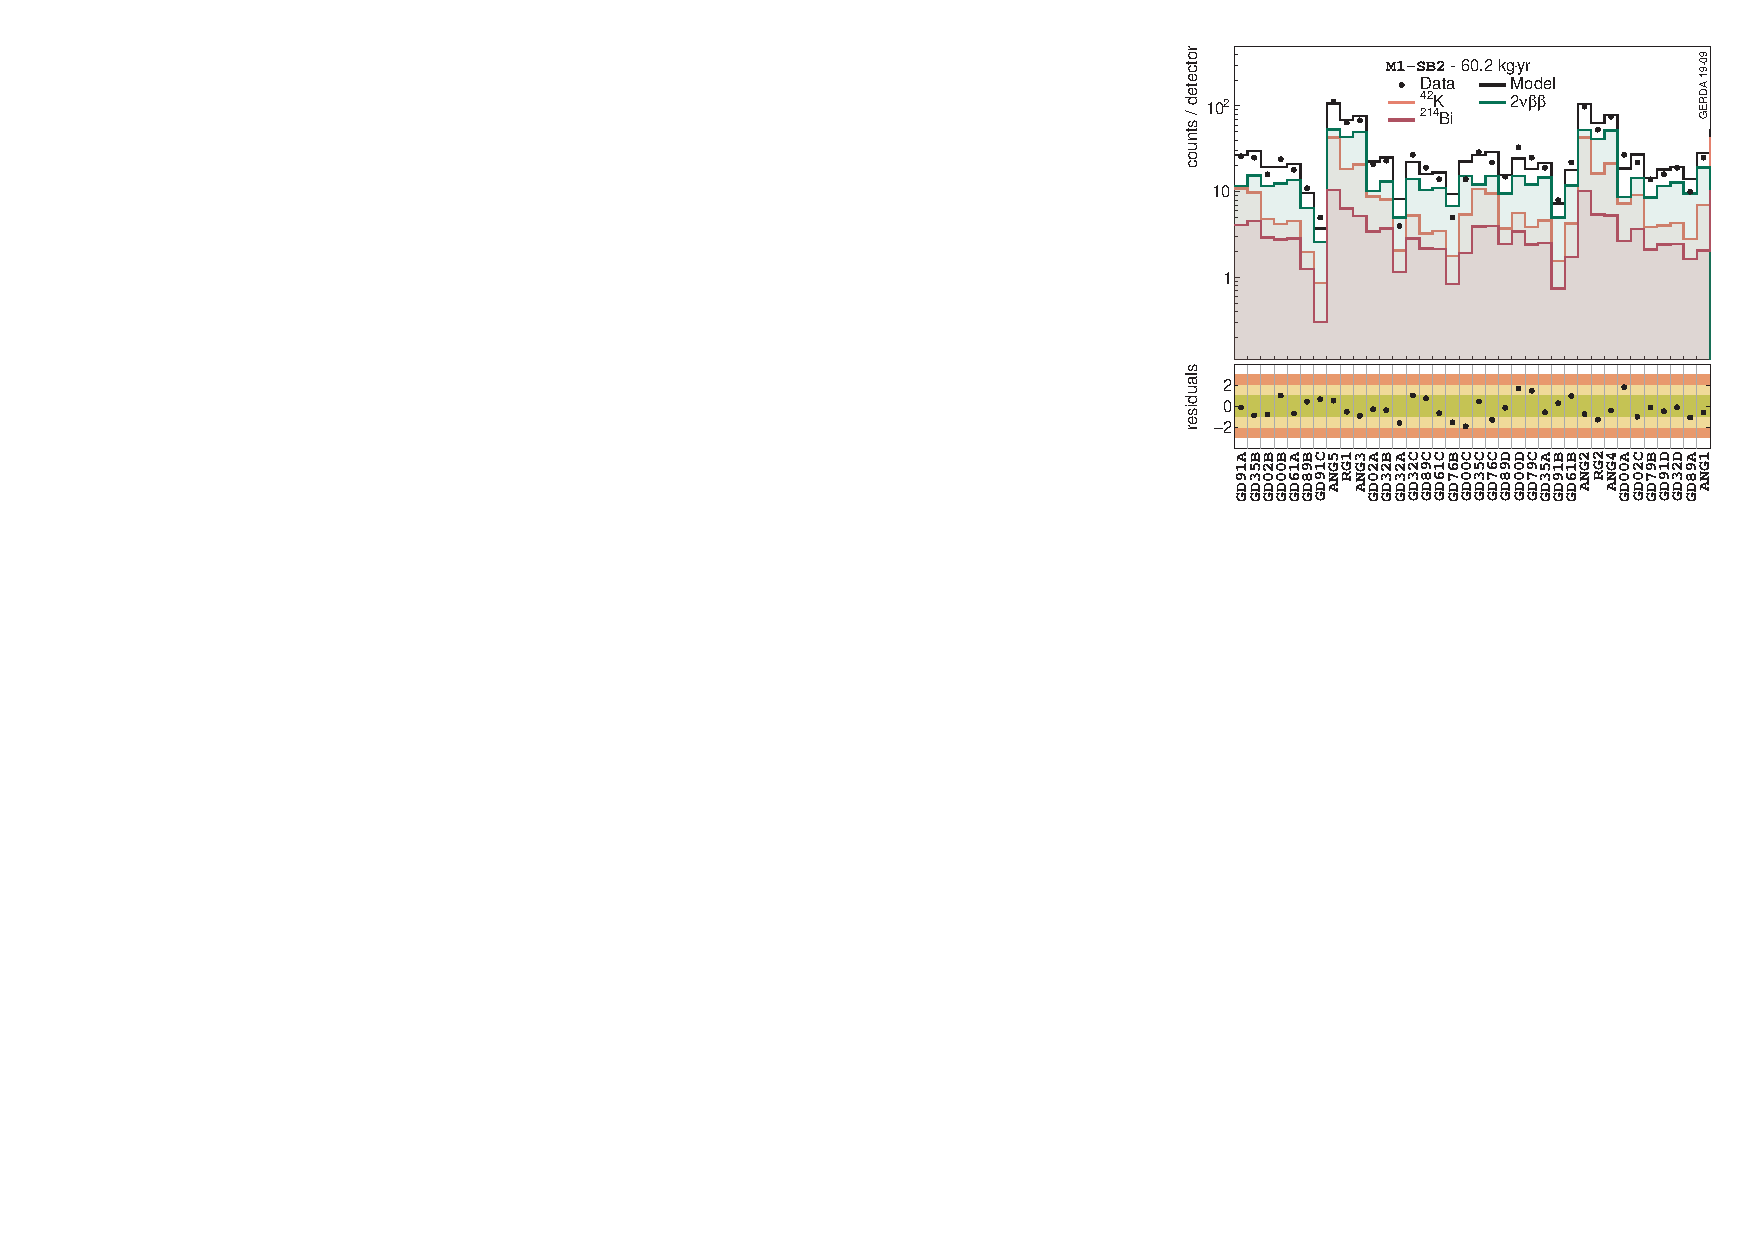
\includegraphics[width=0.45\textwidth]{plots/bkg/raw/ph2/results/kmodel/kmodel-1d-ds3.pdf}\vspace{10pt}
  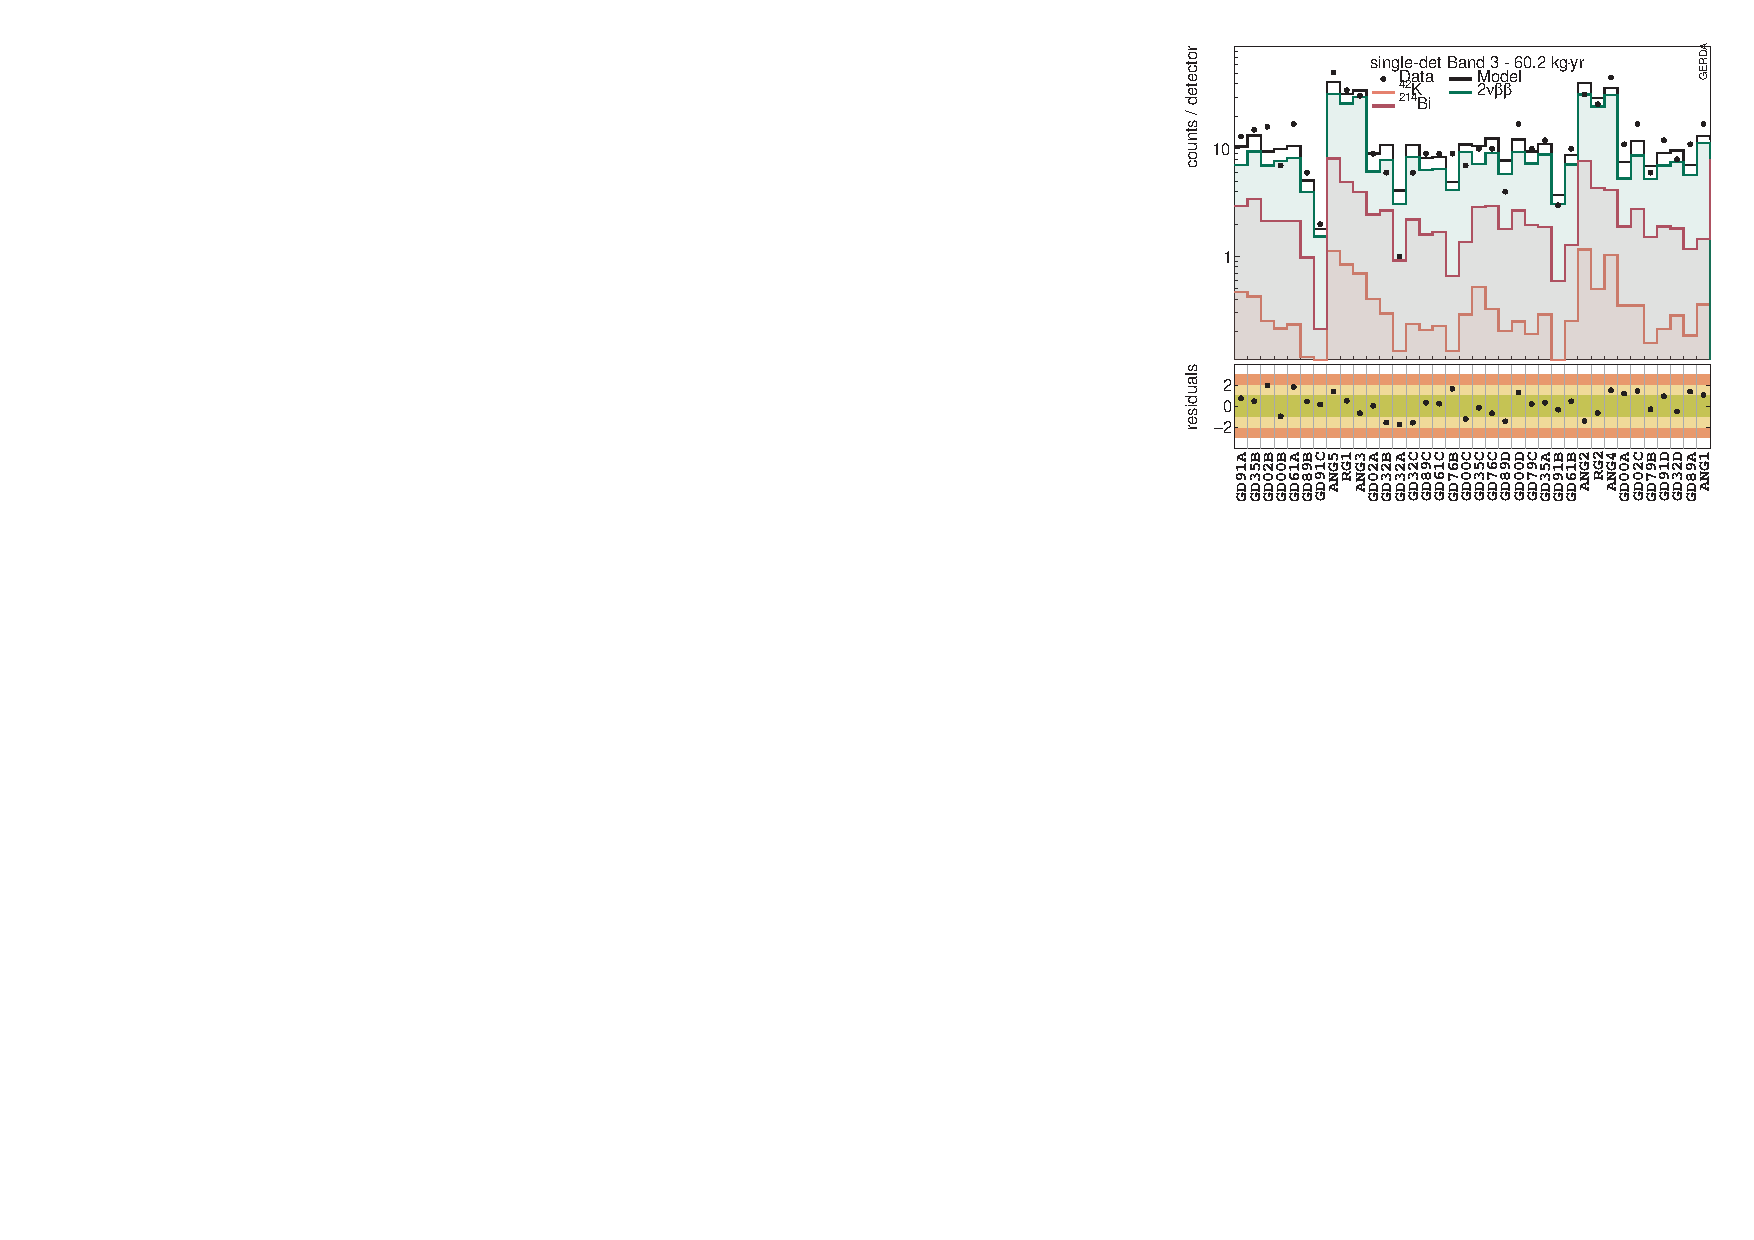
\includegraphics[width=0.45\textwidth]{plots/bkg/raw/ph2/results/kmodel/kmodel-1d-ds4.pdf}
  \begin{minipage}[b][5.3cm][c]{0.45\textwidth}
    \hspace{15pt}%
    \parbox{0.91\textwidth}{%
      \caption{%
        Results of the potassium tracking analysis, single-detector events, base model (see
        \cref{sec:bkg:raw:ph2:kmodel} for details). Some components are merged together to
        ease the visualization. The \emph{close} and \emph{far} keywords refer to the
        background sources location: close to (cables, holders, mini-shrouds) and far from
        (fibers, SiPMs, copper shrouds, front-end electronics) the detector array.
      }\label{fig:bkg:raw:ph2:kmodel:base:results:M1}
    }
  \end{minipage}
\end{figure}

\begin{figure}
  \centering
  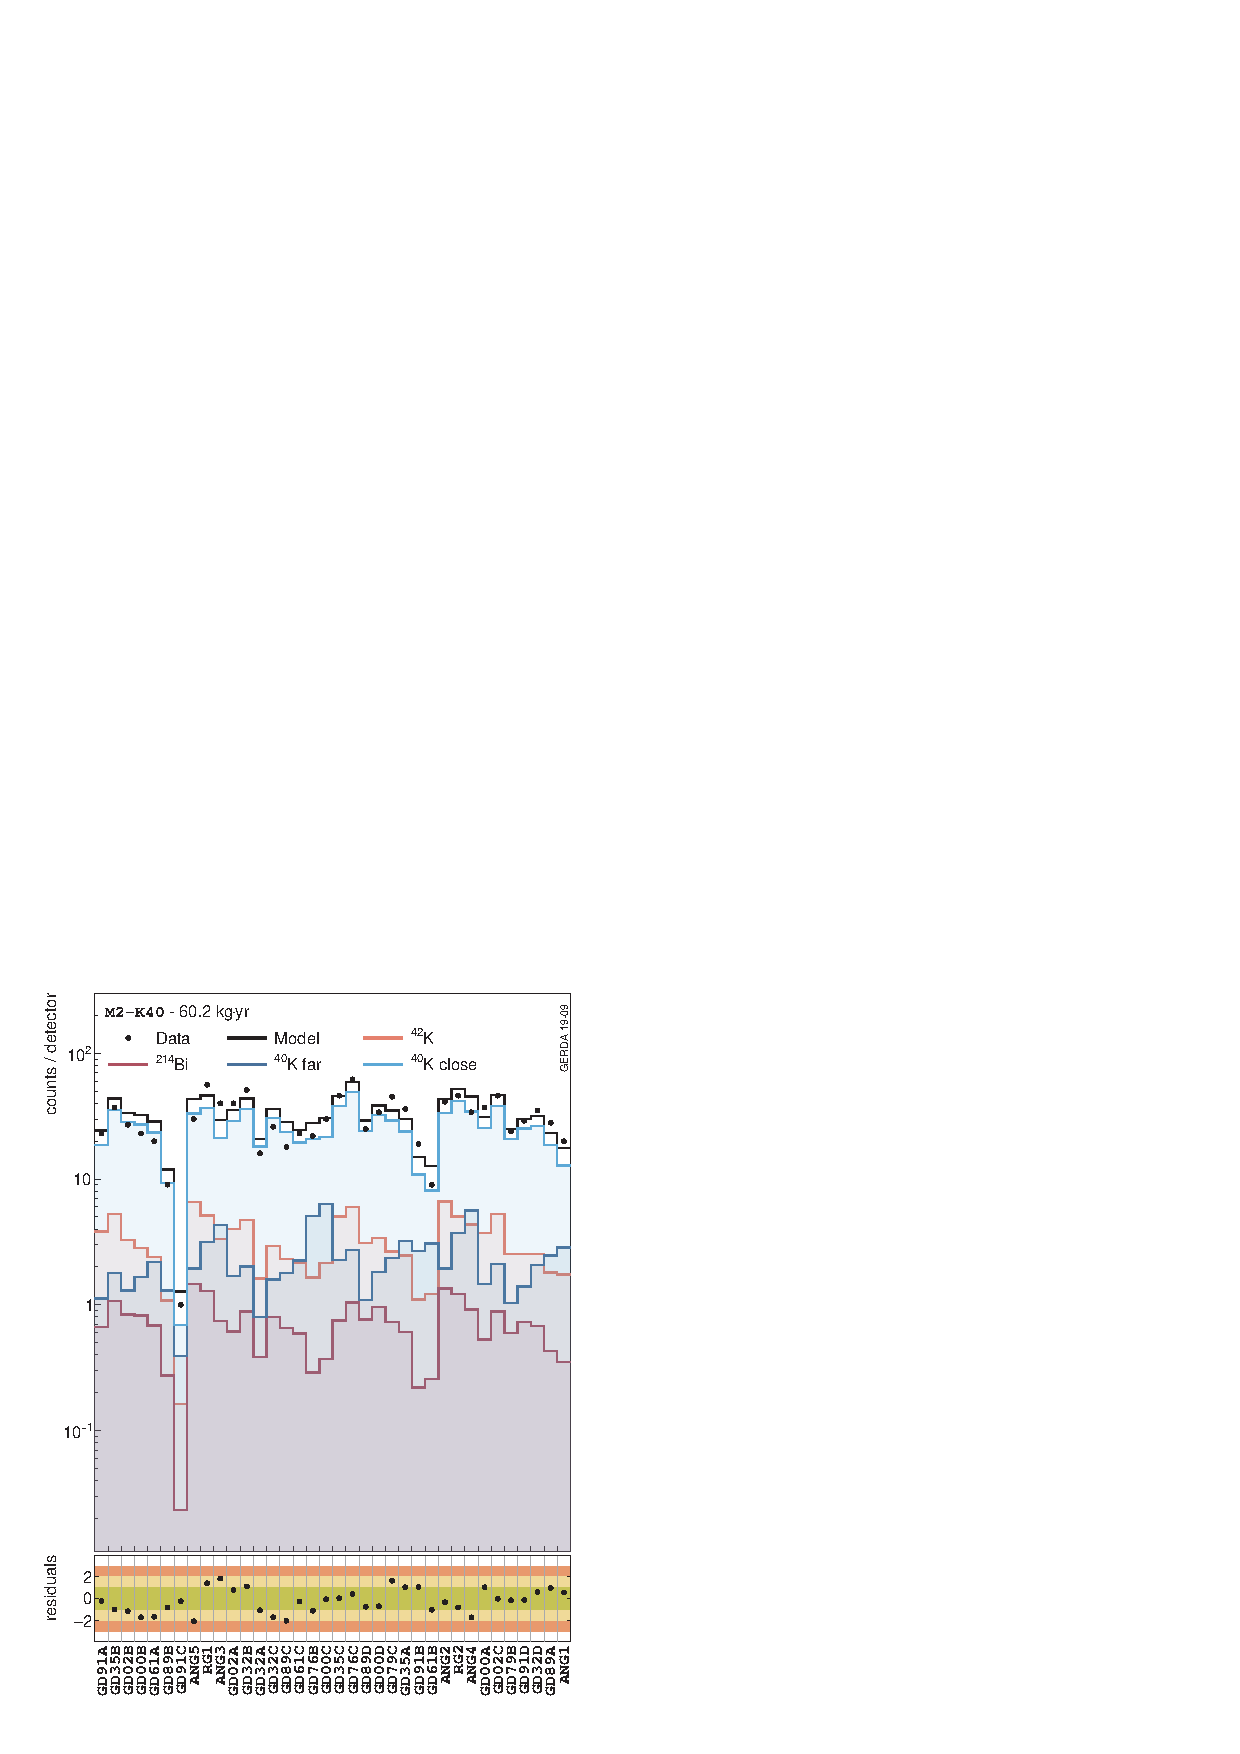
\includegraphics[width=0.45\textwidth]{plots/bkg/raw/ph2/results/kmodel/kmodel-2d-ds5.pdf}
  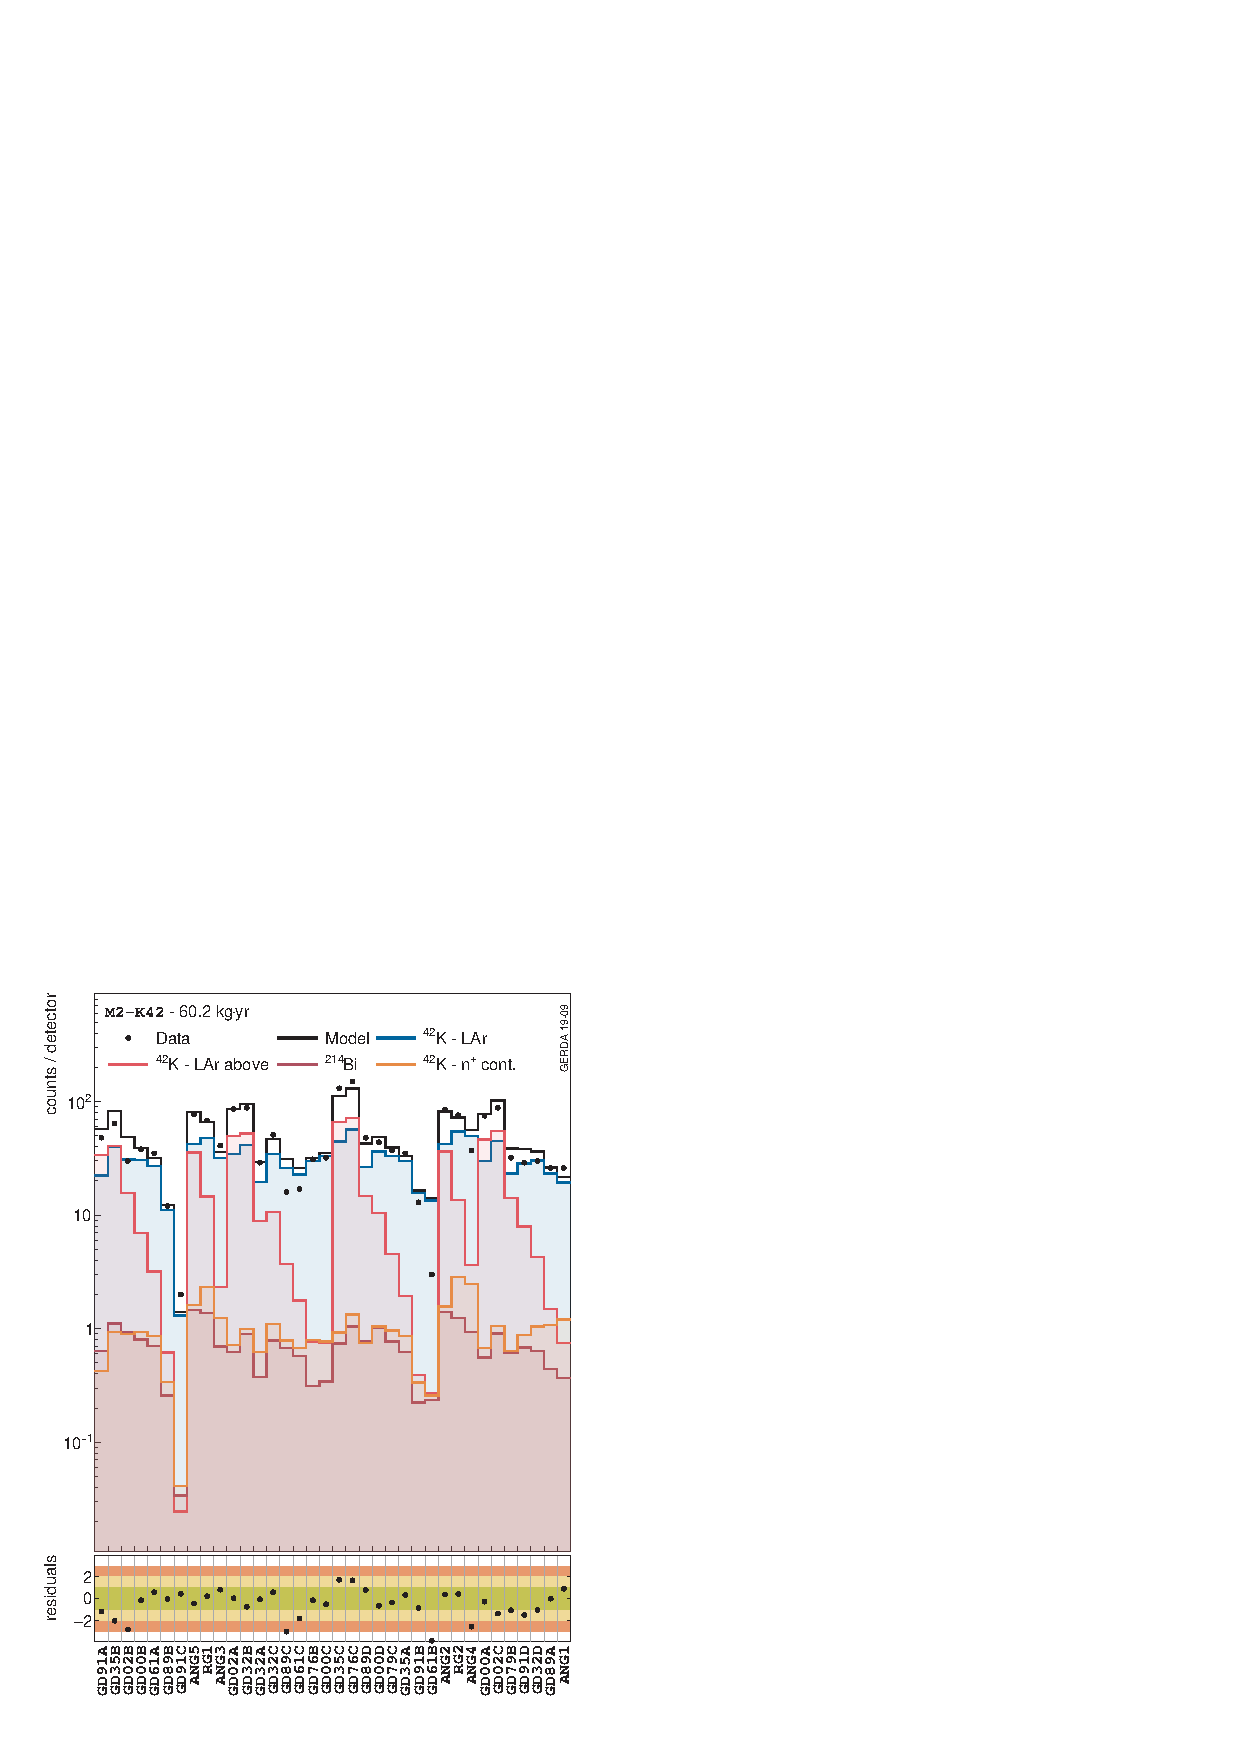
\includegraphics[width=0.45\textwidth]{plots/bkg/raw/ph2/results/kmodel/kmodel-2d-ds6.pdf}\vspace{10pt}
  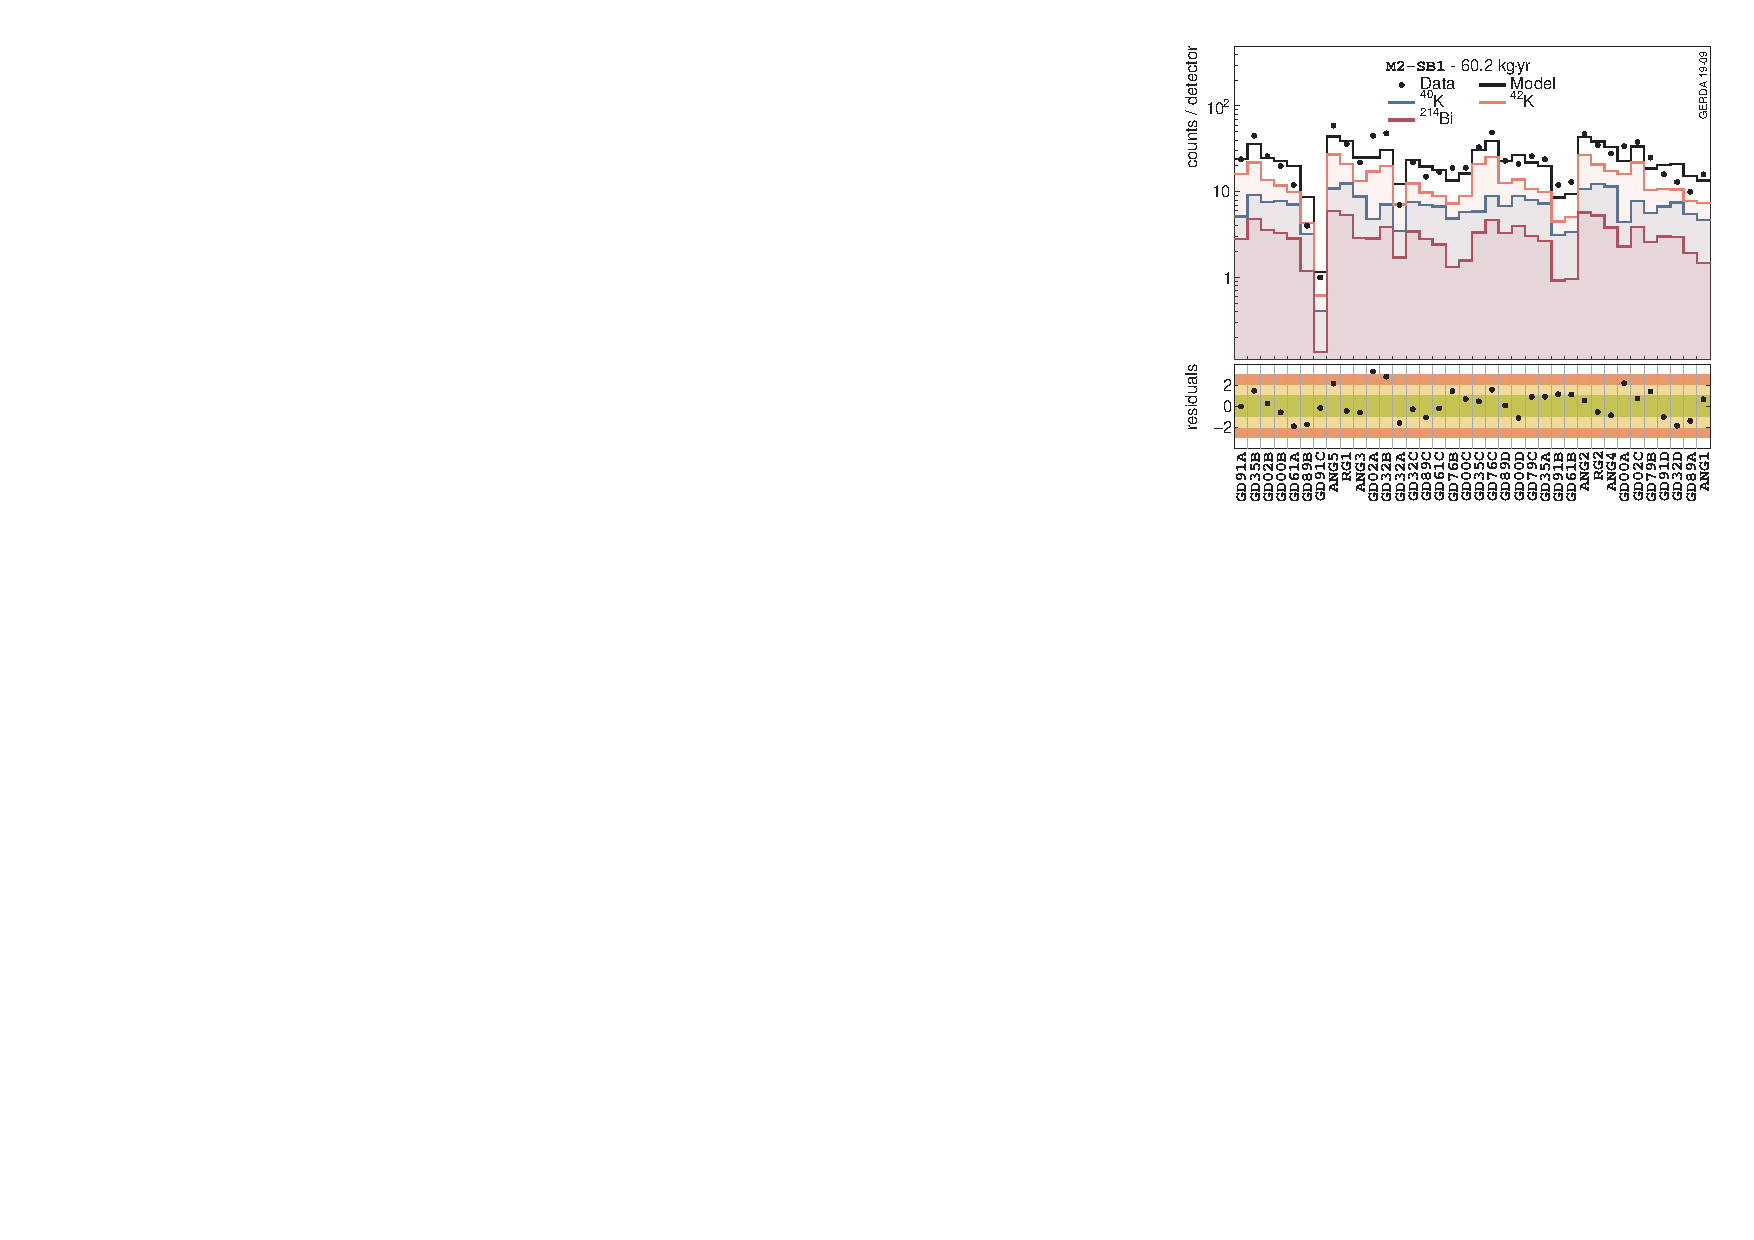
\includegraphics[width=0.45\textwidth]{plots/bkg/raw/ph2/results/kmodel/kmodel-2d-ds7.pdf}
  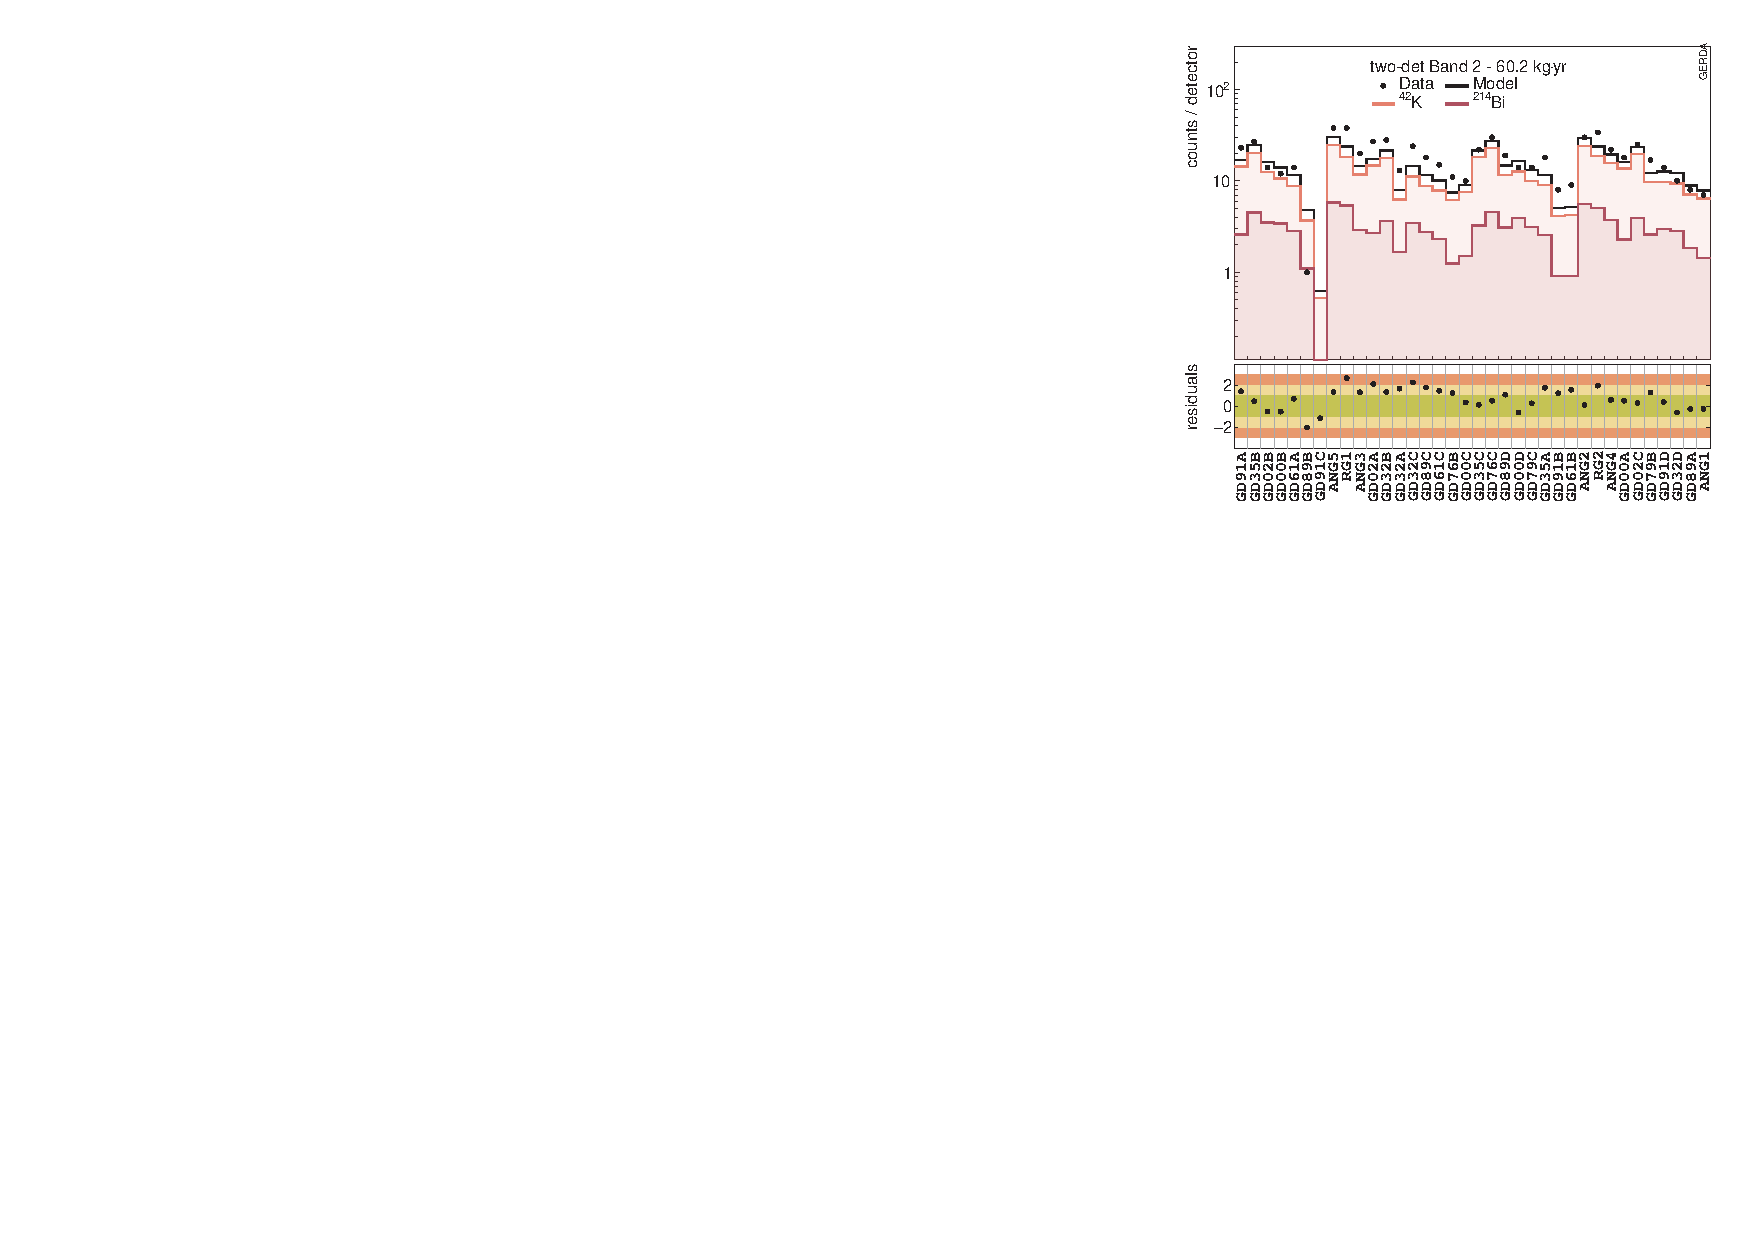
\includegraphics[width=0.45\textwidth]{plots/bkg/raw/ph2/results/kmodel/kmodel-2d-ds8.pdf}\vspace{10pt}
  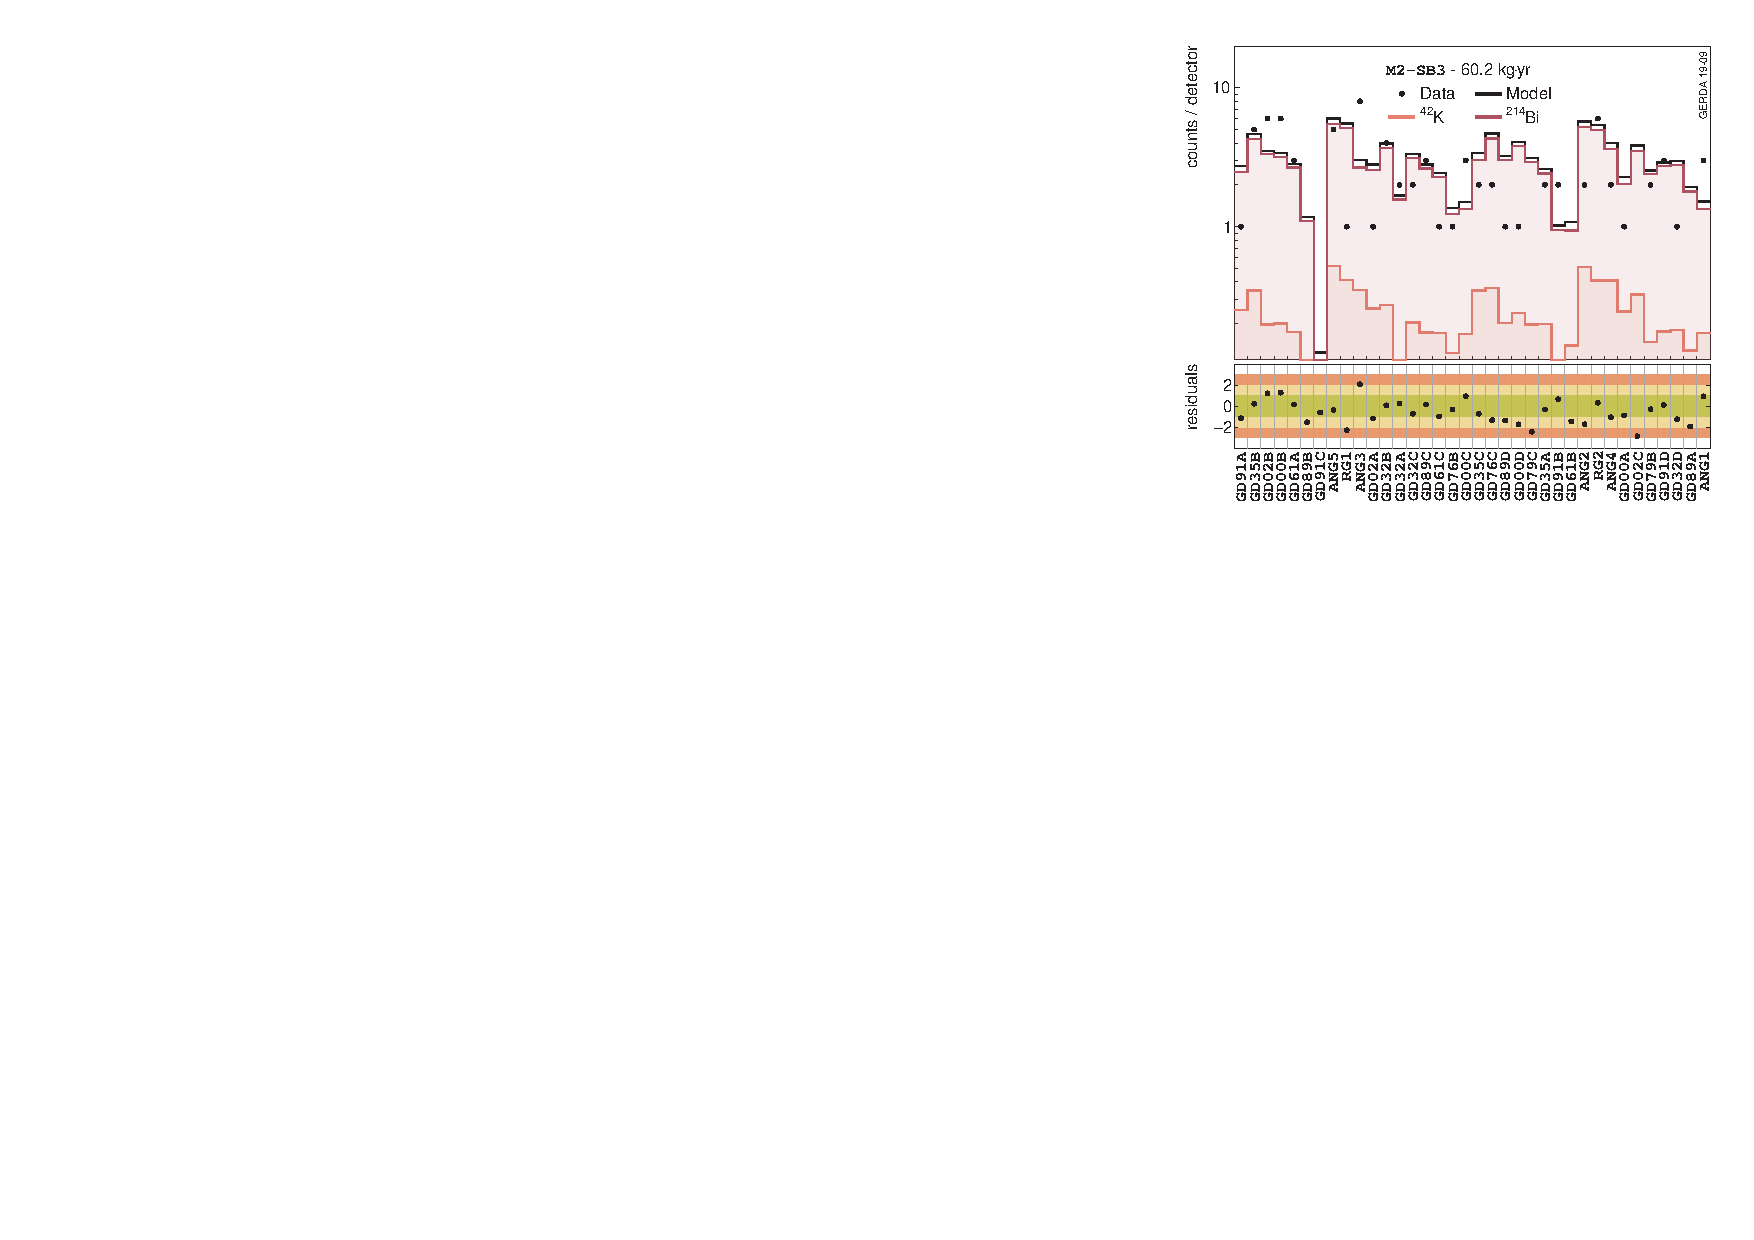
\includegraphics[width=0.45\textwidth]{plots/bkg/raw/ph2/results/kmodel/kmodel-2d-ds9.pdf}
  \begin{minipage}[b][5.3cm][c]{0.45\textwidth}
    \hspace{15pt}%
    \parbox{0.91\textwidth}{%
      \caption{%
        Results of the potassium tracking analysis, two-detector events, base model (see
        \cref{sec:bkg:raw:ph2:kmodel} for details). To visualize the two-detector data the
        sum of the projections on the two domain axes is shown. Some components are merged
        together to ease the visualization. The \emph{close} and \emph{far} keywords refer
        to the background sources location: close to (cables, holders, mini-shrouds) and far
        from (fibers, SiPMs, copper shrouds, front-end electronics) the detector array.
      }\label{fig:bkg:raw:ph2:kmodel:base:results:M2}
    }
  \end{minipage}
\end{figure}

\begin{figure}
  \centering
  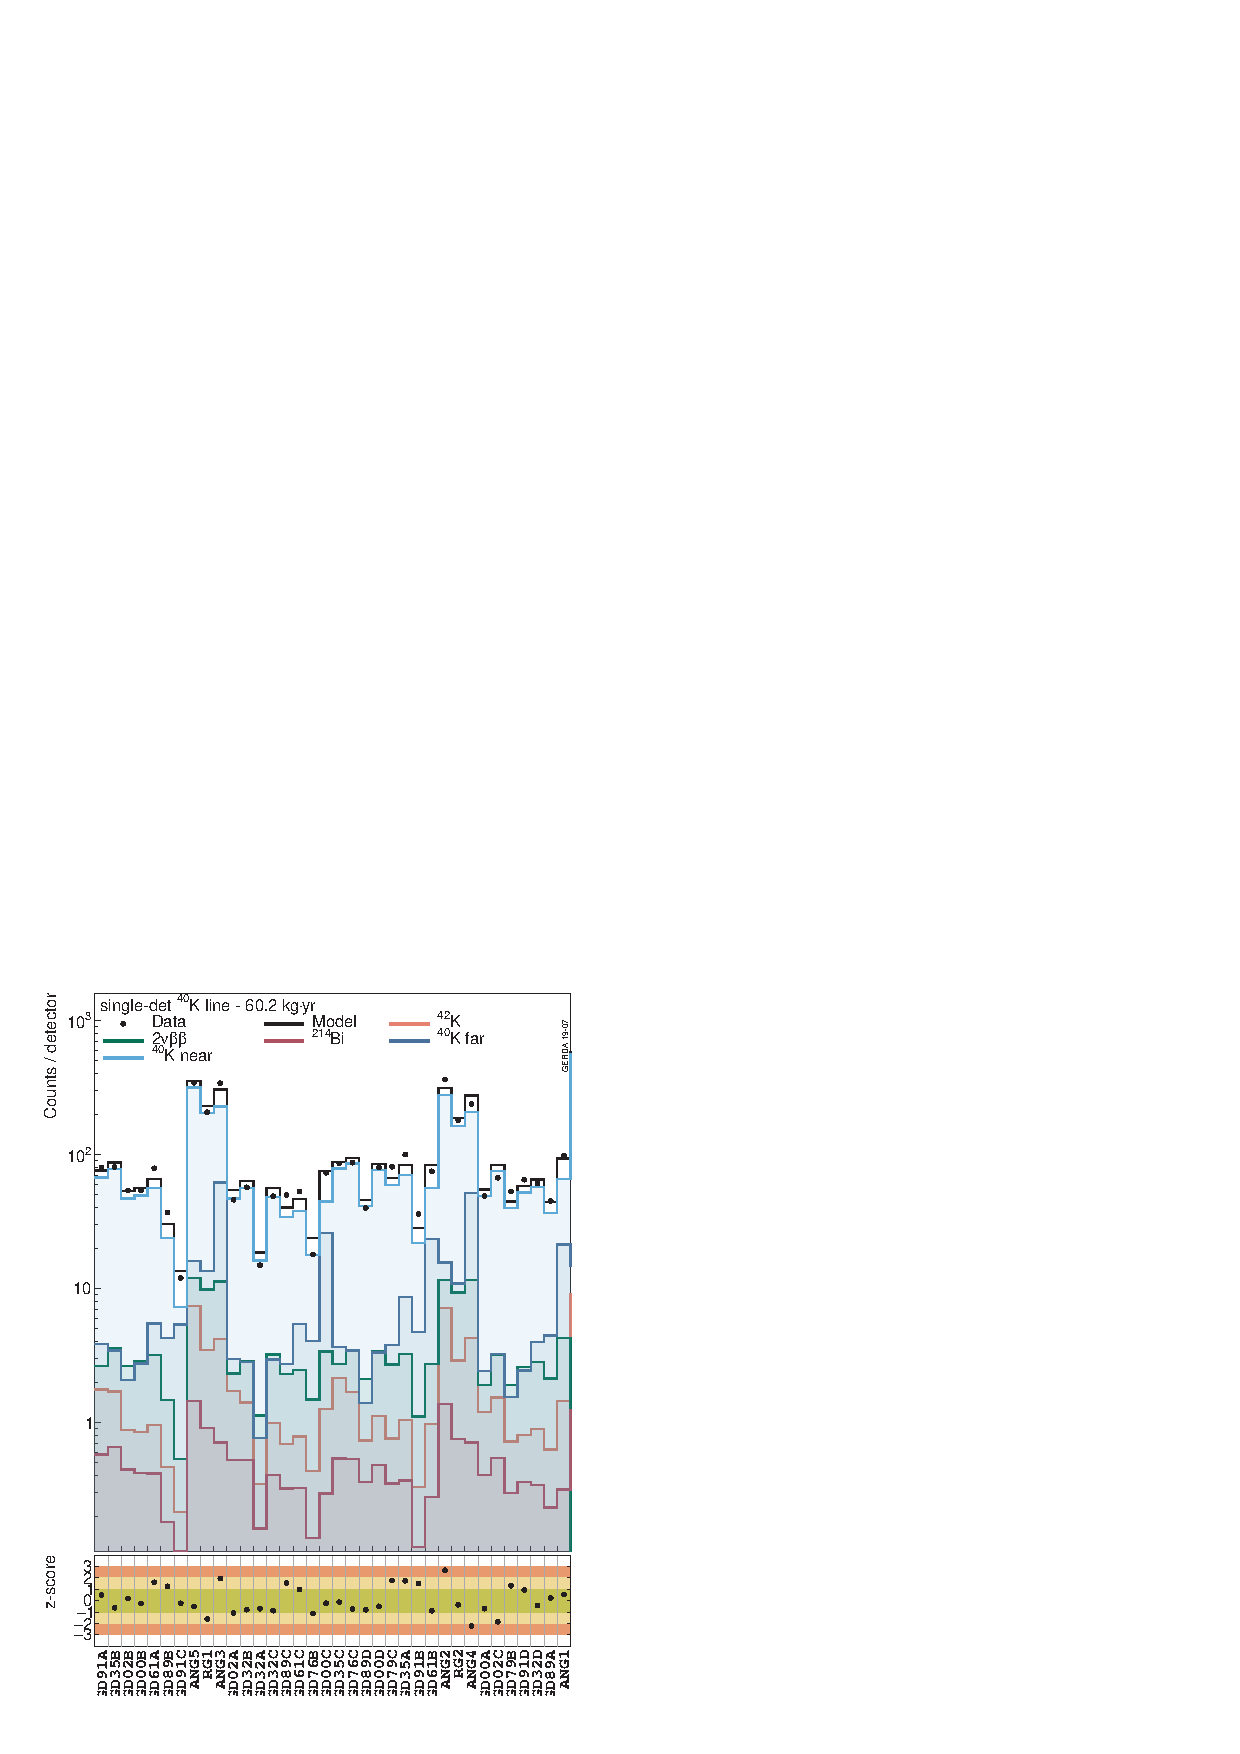
\includegraphics[width=0.45\textwidth]{plots/bkg/raw/ph2/results/kmodel/kmodel-1d-ds0-complete.pdf}
  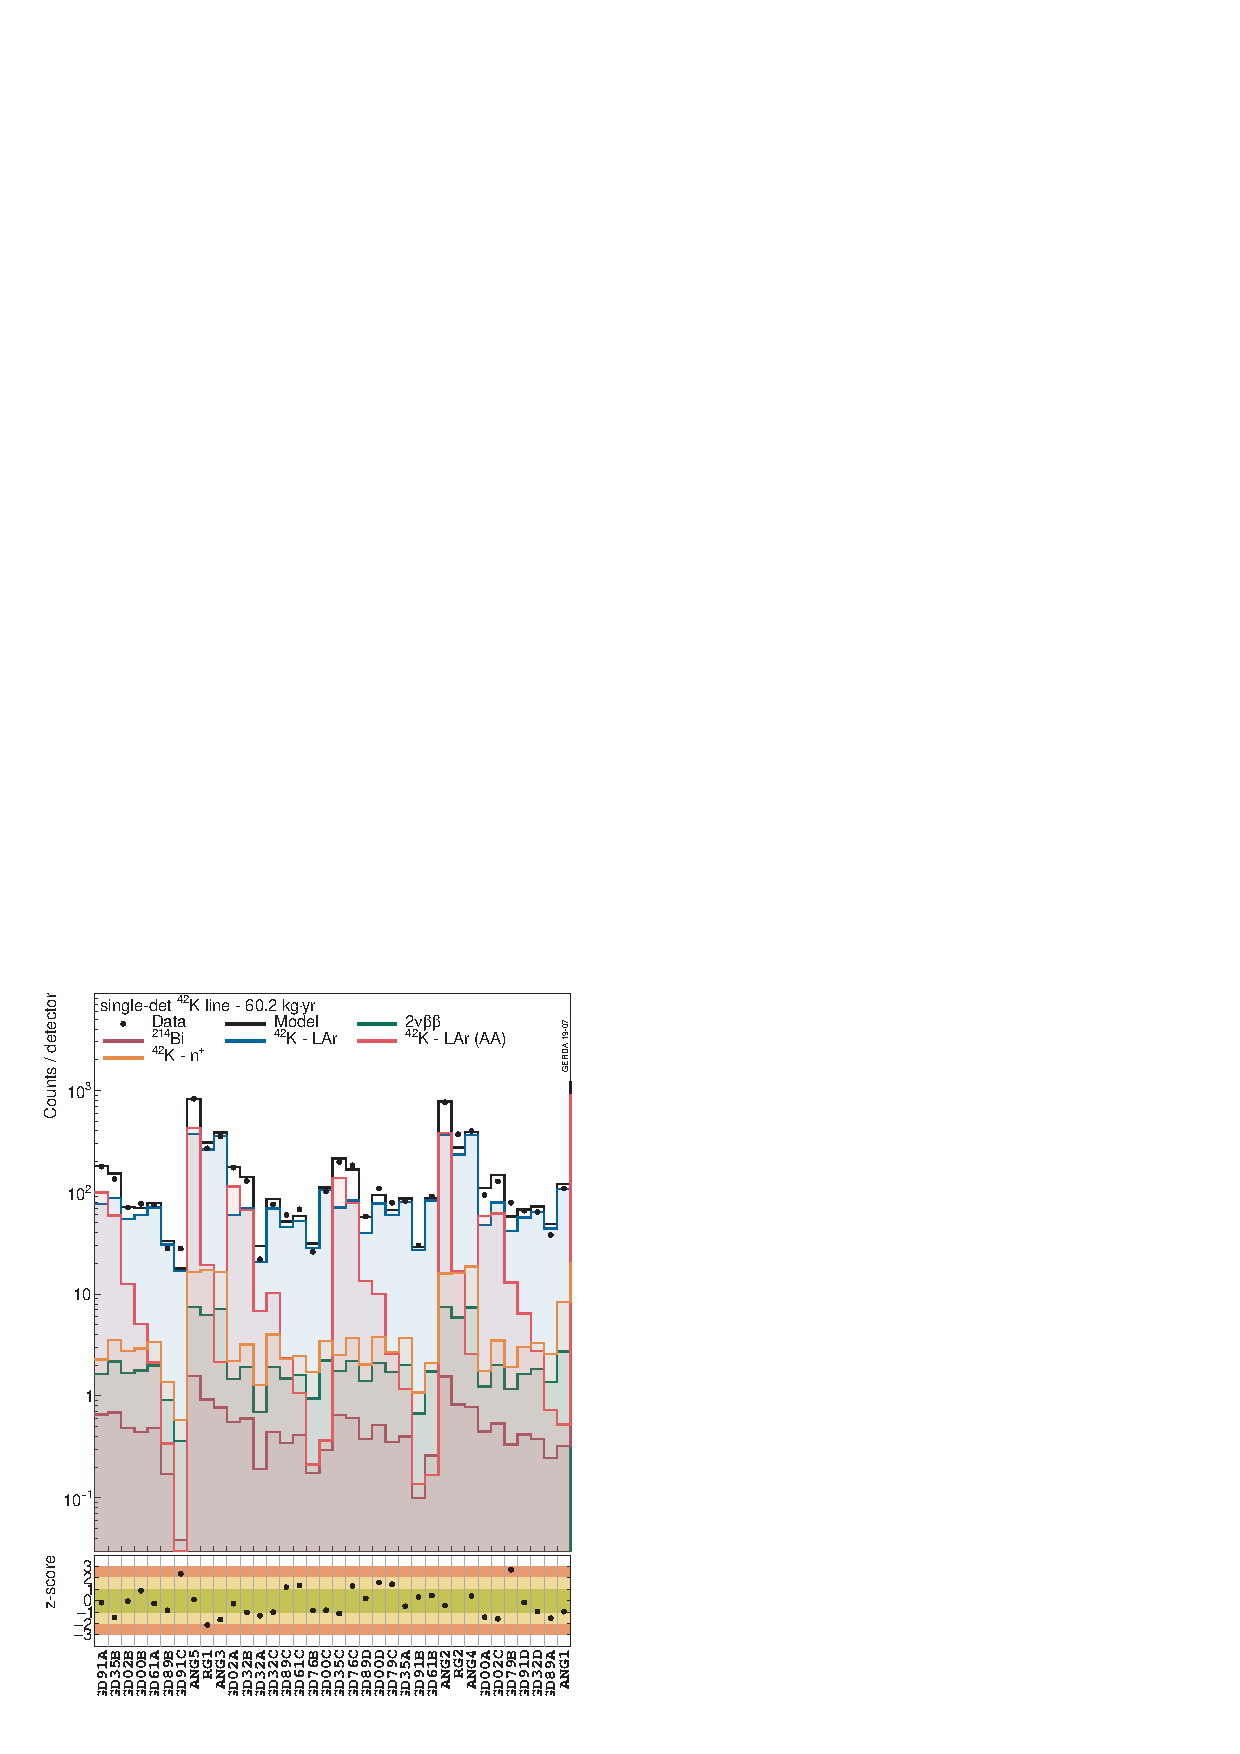
\includegraphics[width=0.45\textwidth]{plots/bkg/raw/ph2/results/kmodel/kmodel-1d-ds1-complete.pdf}\vspace{10pt}
  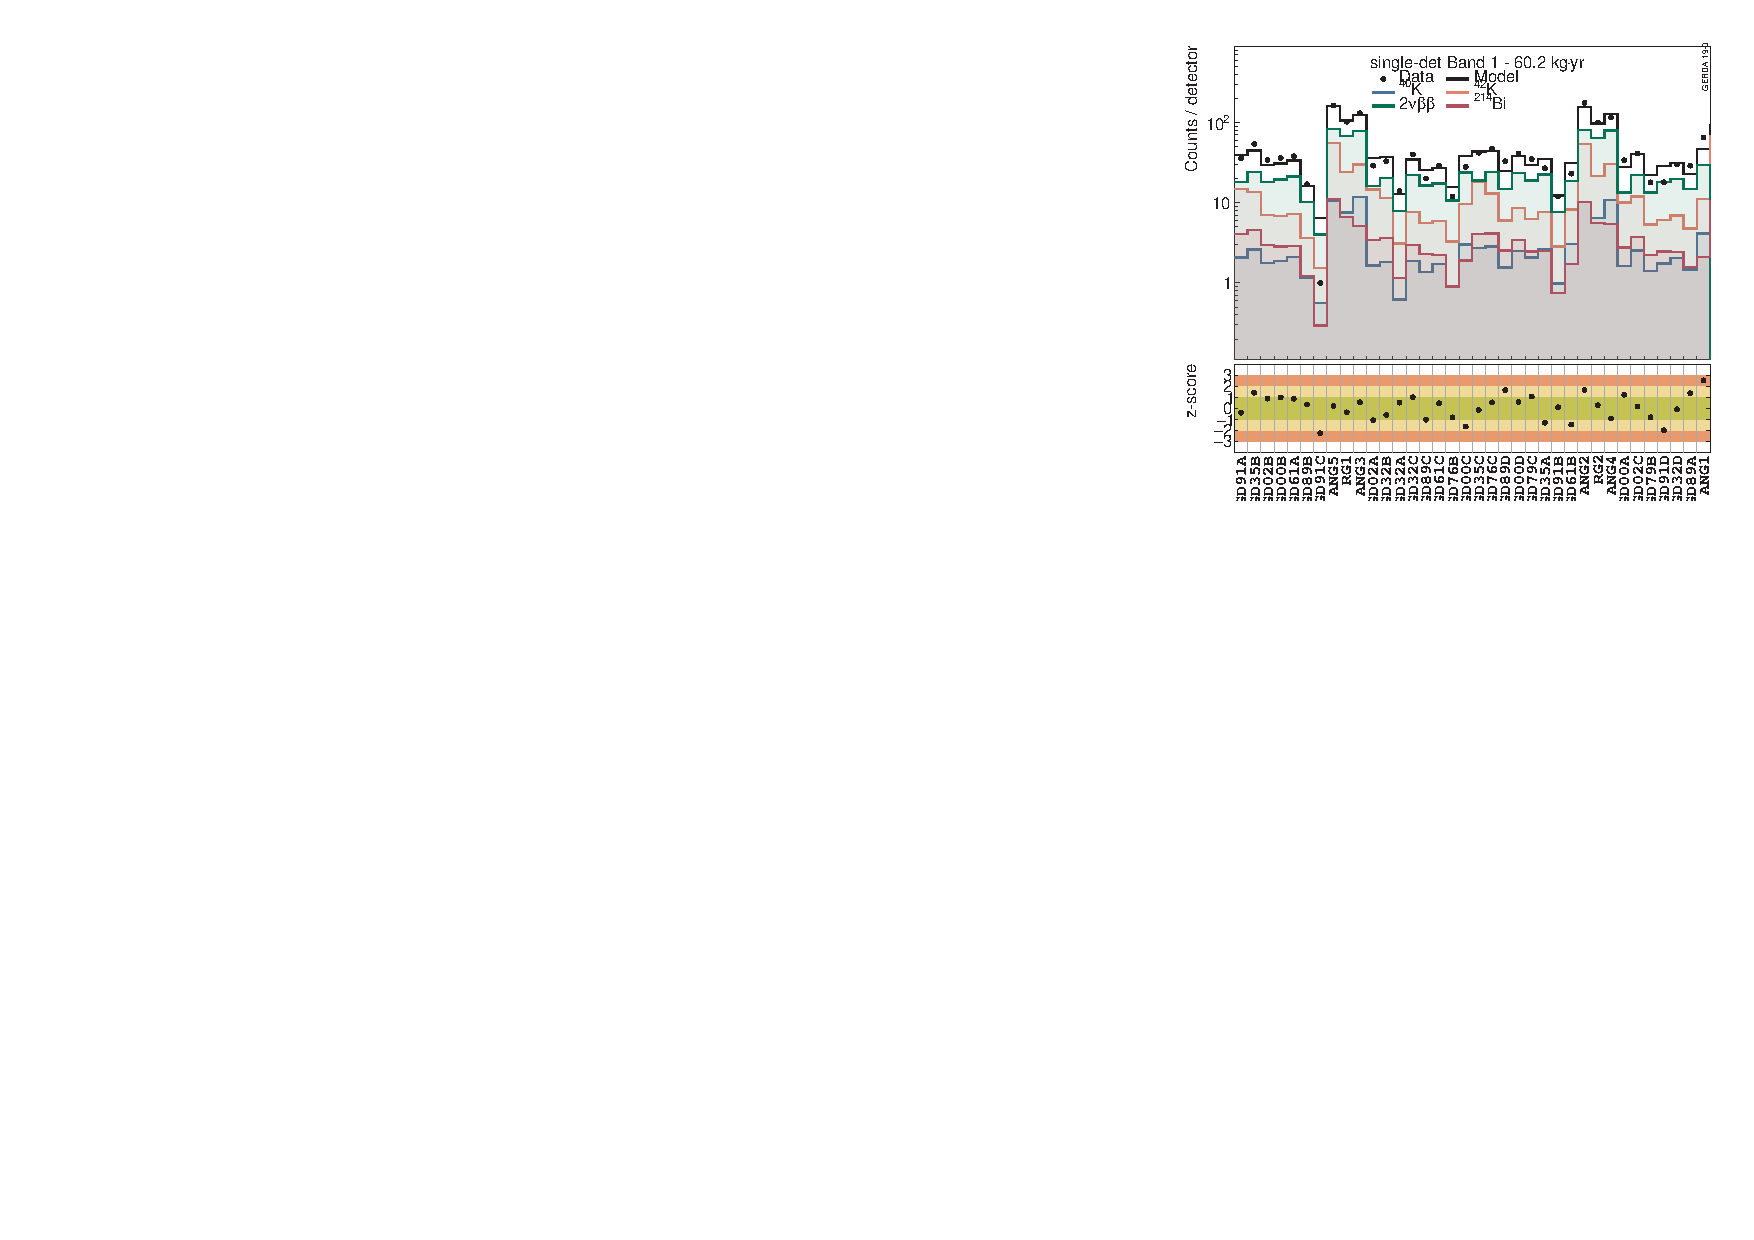
\includegraphics[width=0.45\textwidth]{plots/bkg/raw/ph2/results/kmodel/kmodel-1d-ds2-complete.pdf}
  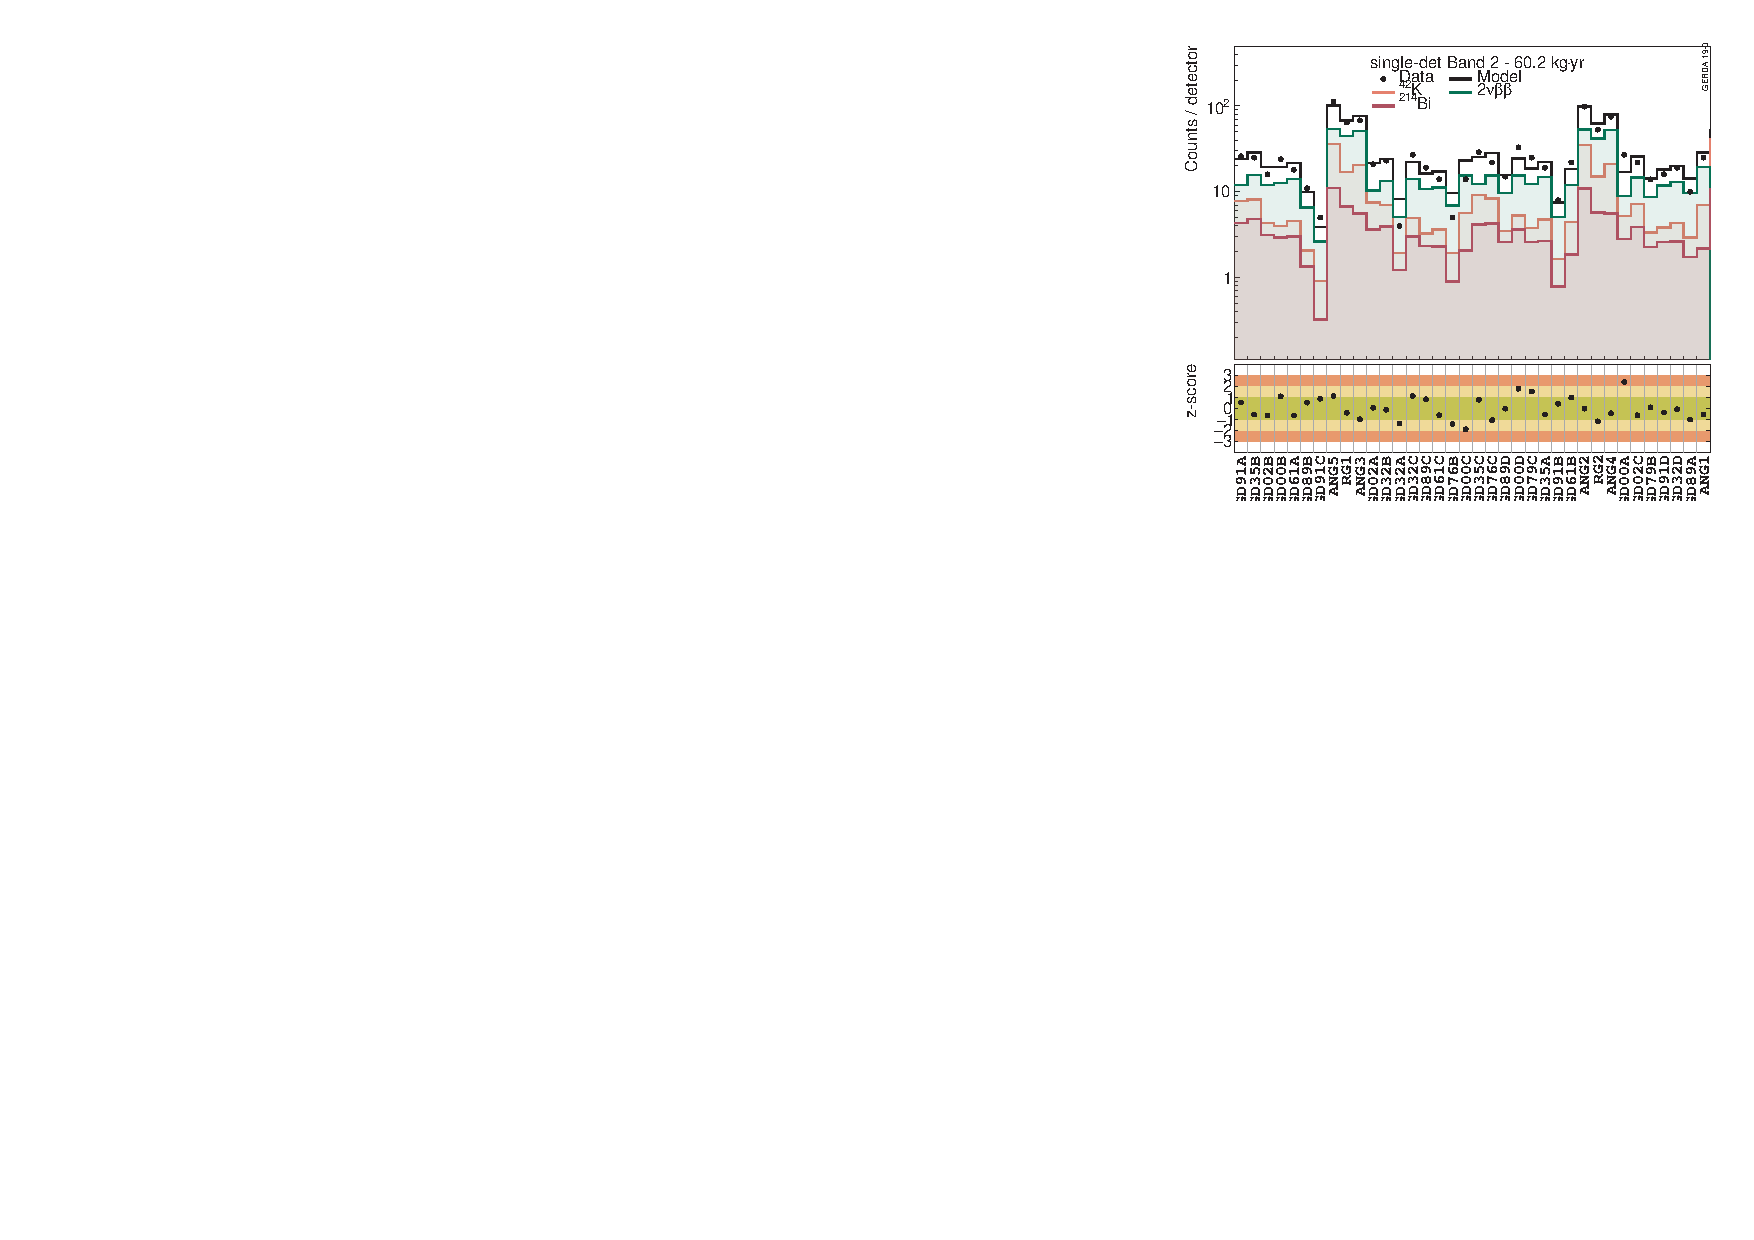
\includegraphics[width=0.45\textwidth]{plots/bkg/raw/ph2/results/kmodel/kmodel-1d-ds3-complete.pdf}\vspace{10pt}
  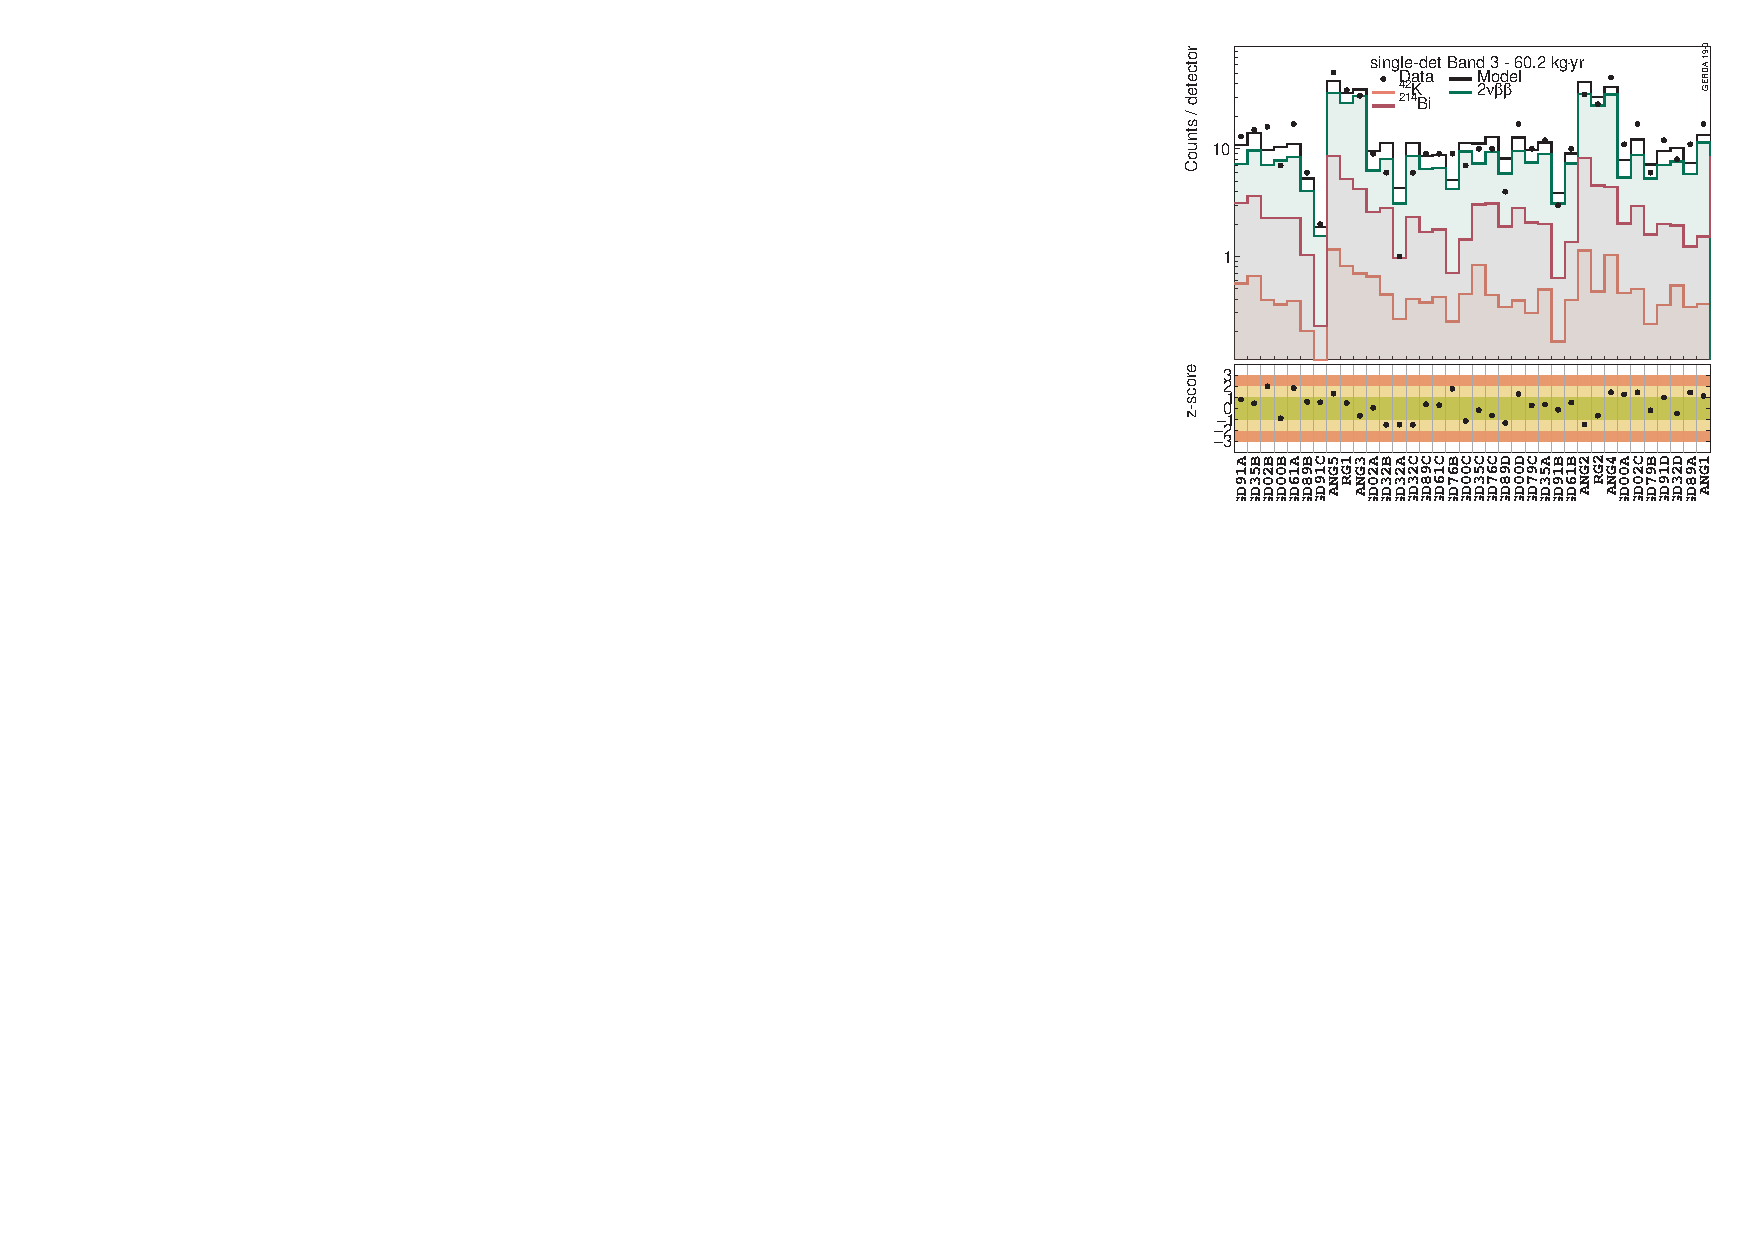
\includegraphics[width=0.45\textwidth]{plots/bkg/raw/ph2/results/kmodel/kmodel-1d-ds4-complete.pdf}
  \begin{minipage}[b][5.3cm][c]{0.45\textwidth}
    \hspace{15pt}%
    \parbox{0.91\textwidth}{%
      \caption{%
        Results of the potassium tracking analysis, single-detector events, extended model (see
        \cref{sec:bkg:raw:ph2:kmodel} for details). Some components are merged together to
        ease the visualization. The \emph{close} and \emph{far} keywords refer to the
        background sources location: close to (cables, holders, mini-shrouds) and far from
        (fibers, SiPMs, copper shrouds, front-end electronics) the detector array.
      }\label{fig:bkg:raw:ph2:kmodel:extended:results:M1}
    }
  \end{minipage}
\end{figure}

\begin{figure}
  \centering
  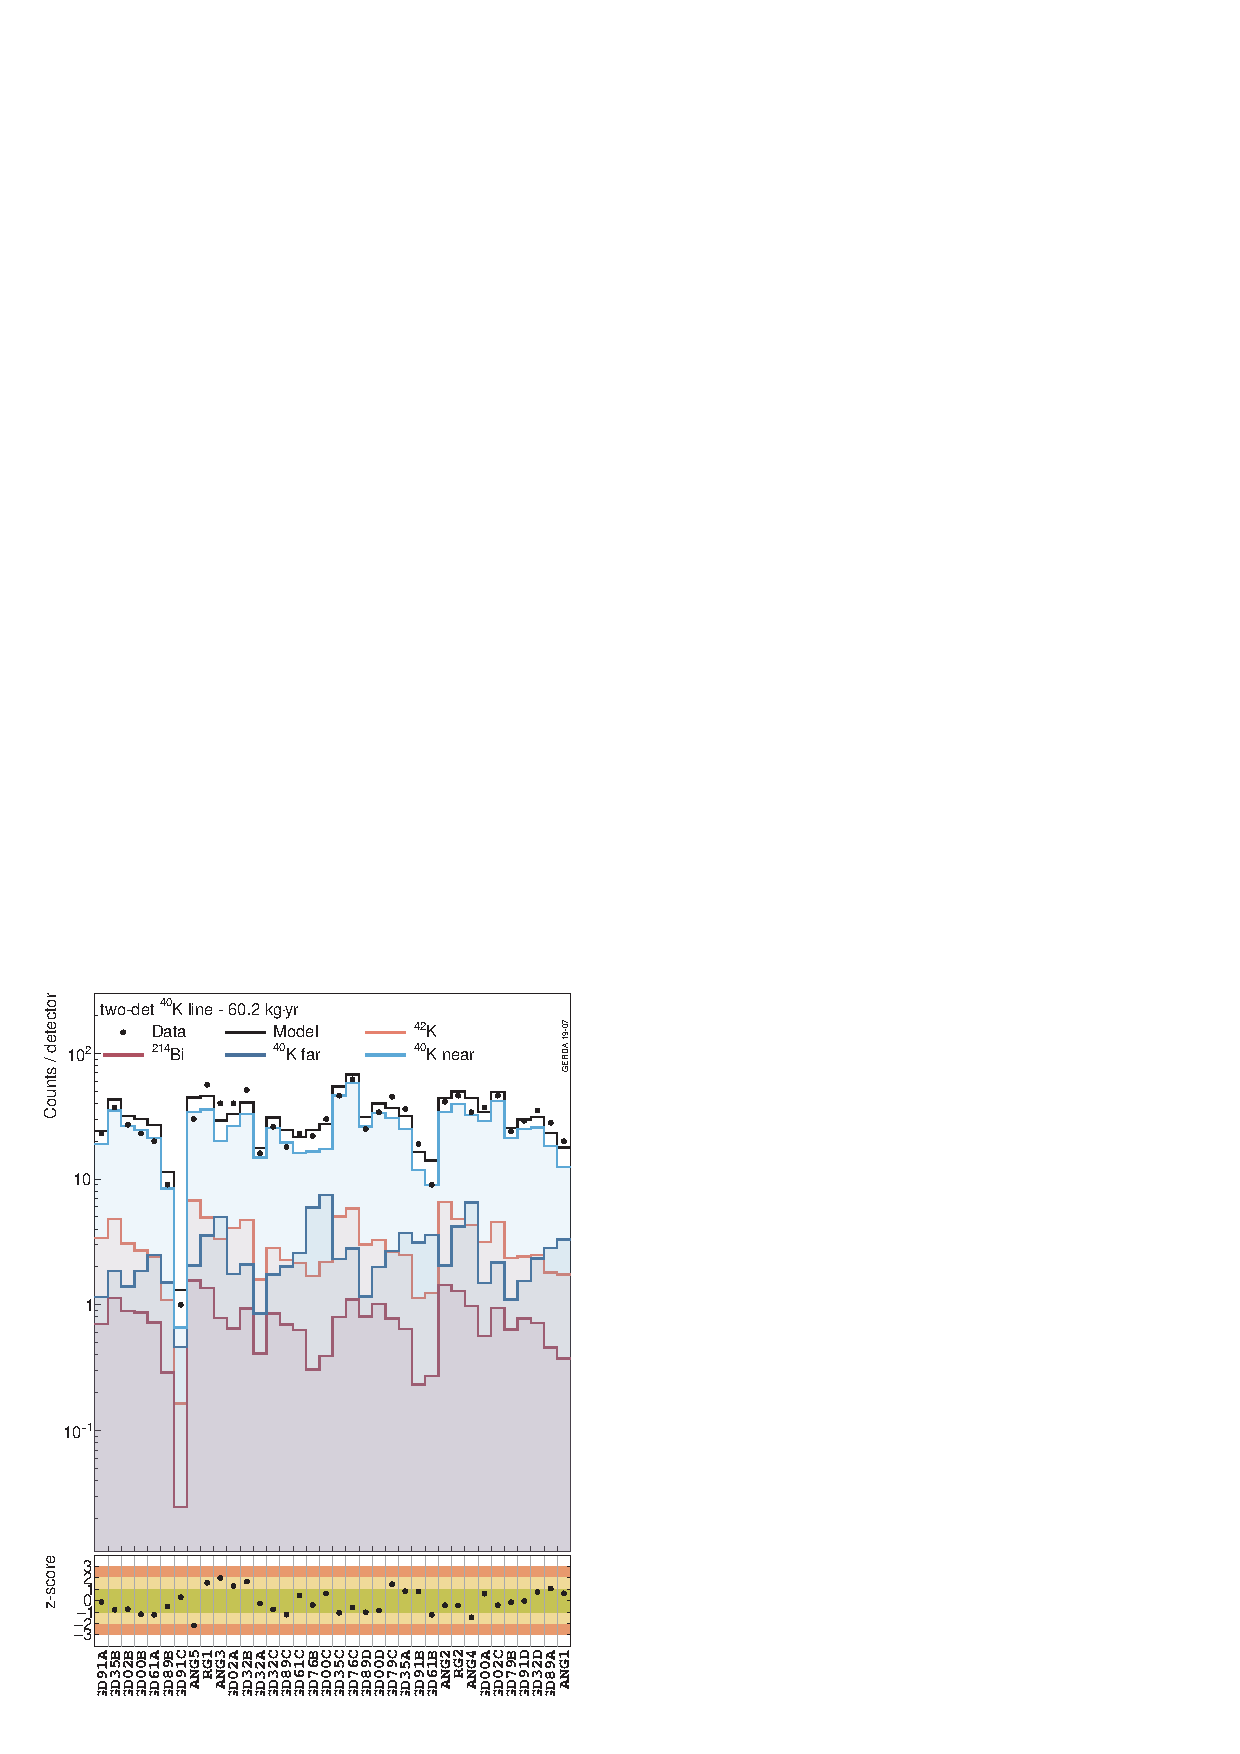
\includegraphics[width=0.45\textwidth]{plots/bkg/raw/ph2/results/kmodel/kmodel-2d-ds5-complete.pdf}
  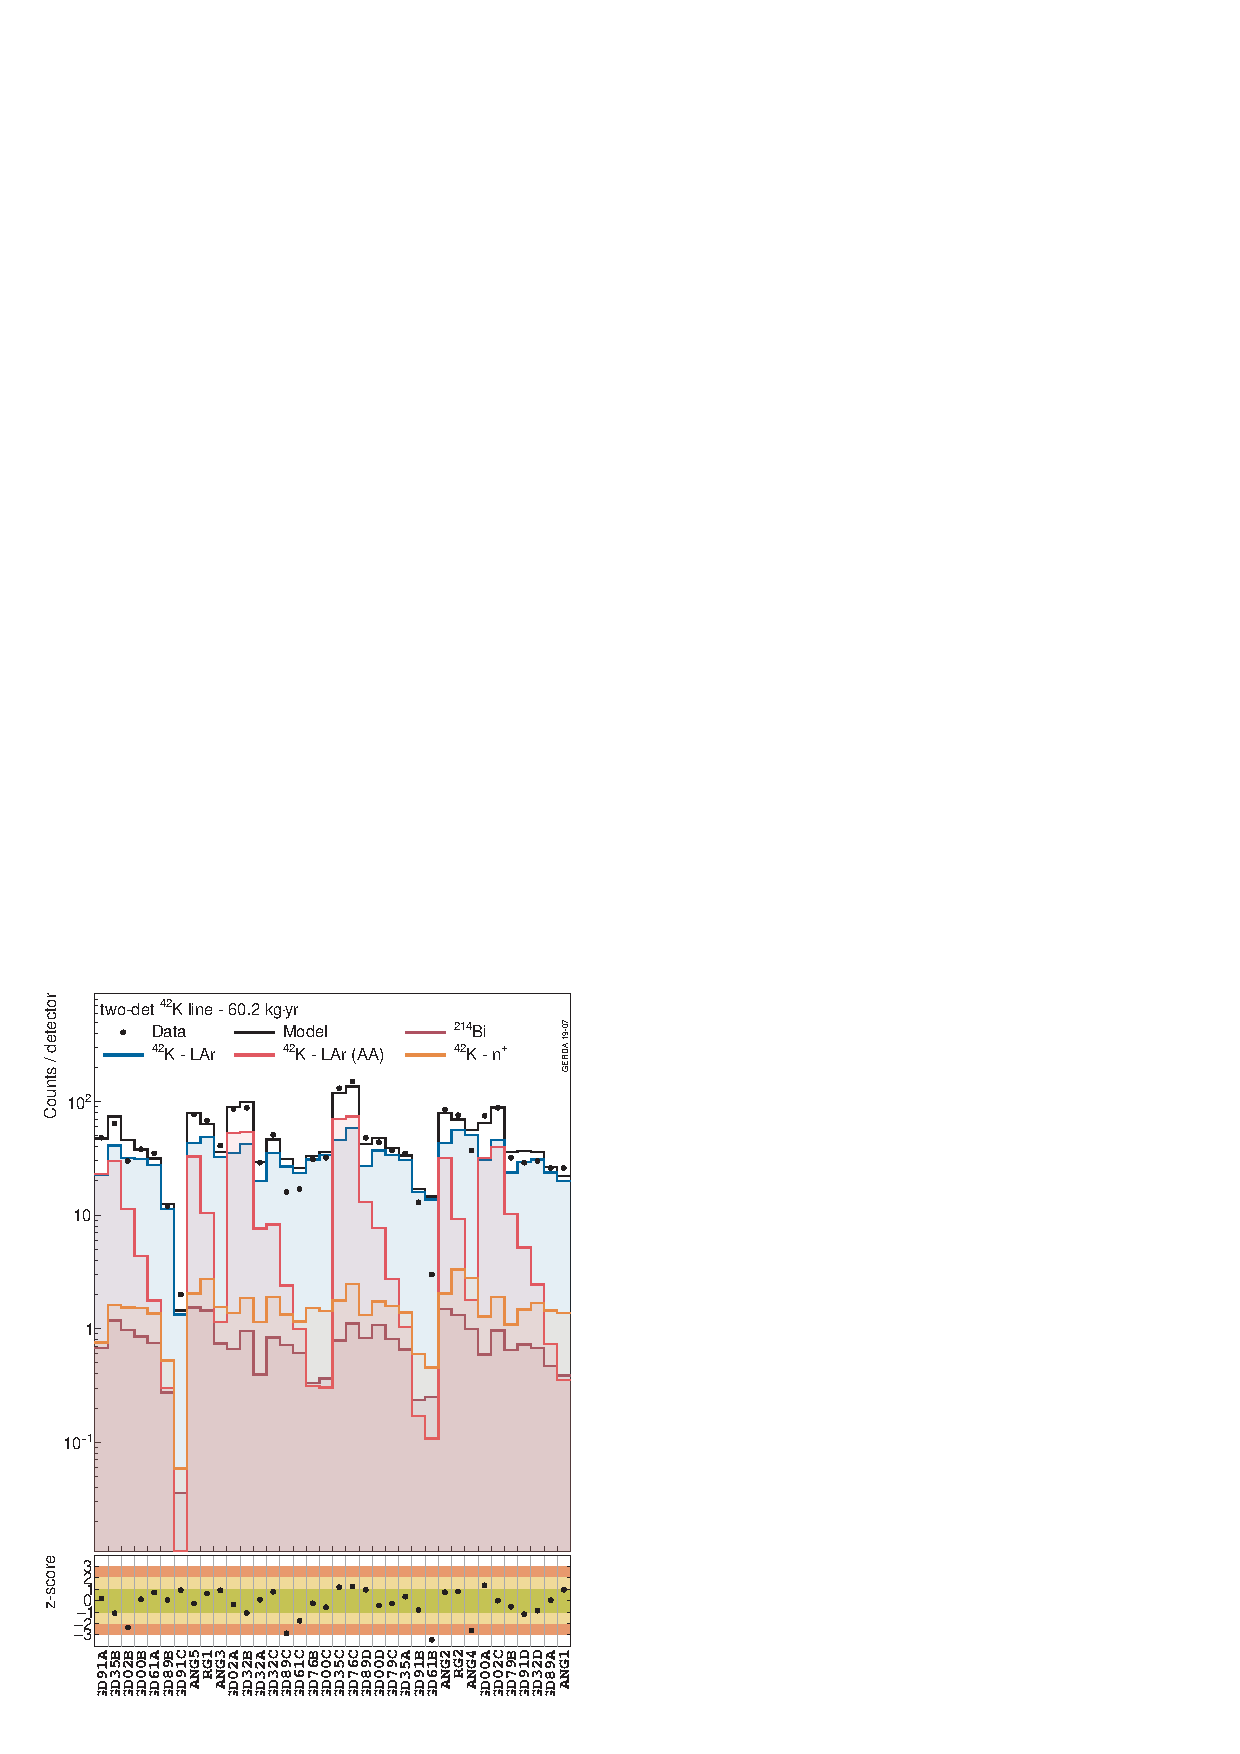
\includegraphics[width=0.45\textwidth]{plots/bkg/raw/ph2/results/kmodel/kmodel-2d-ds6-complete.pdf}\vspace{10pt}
  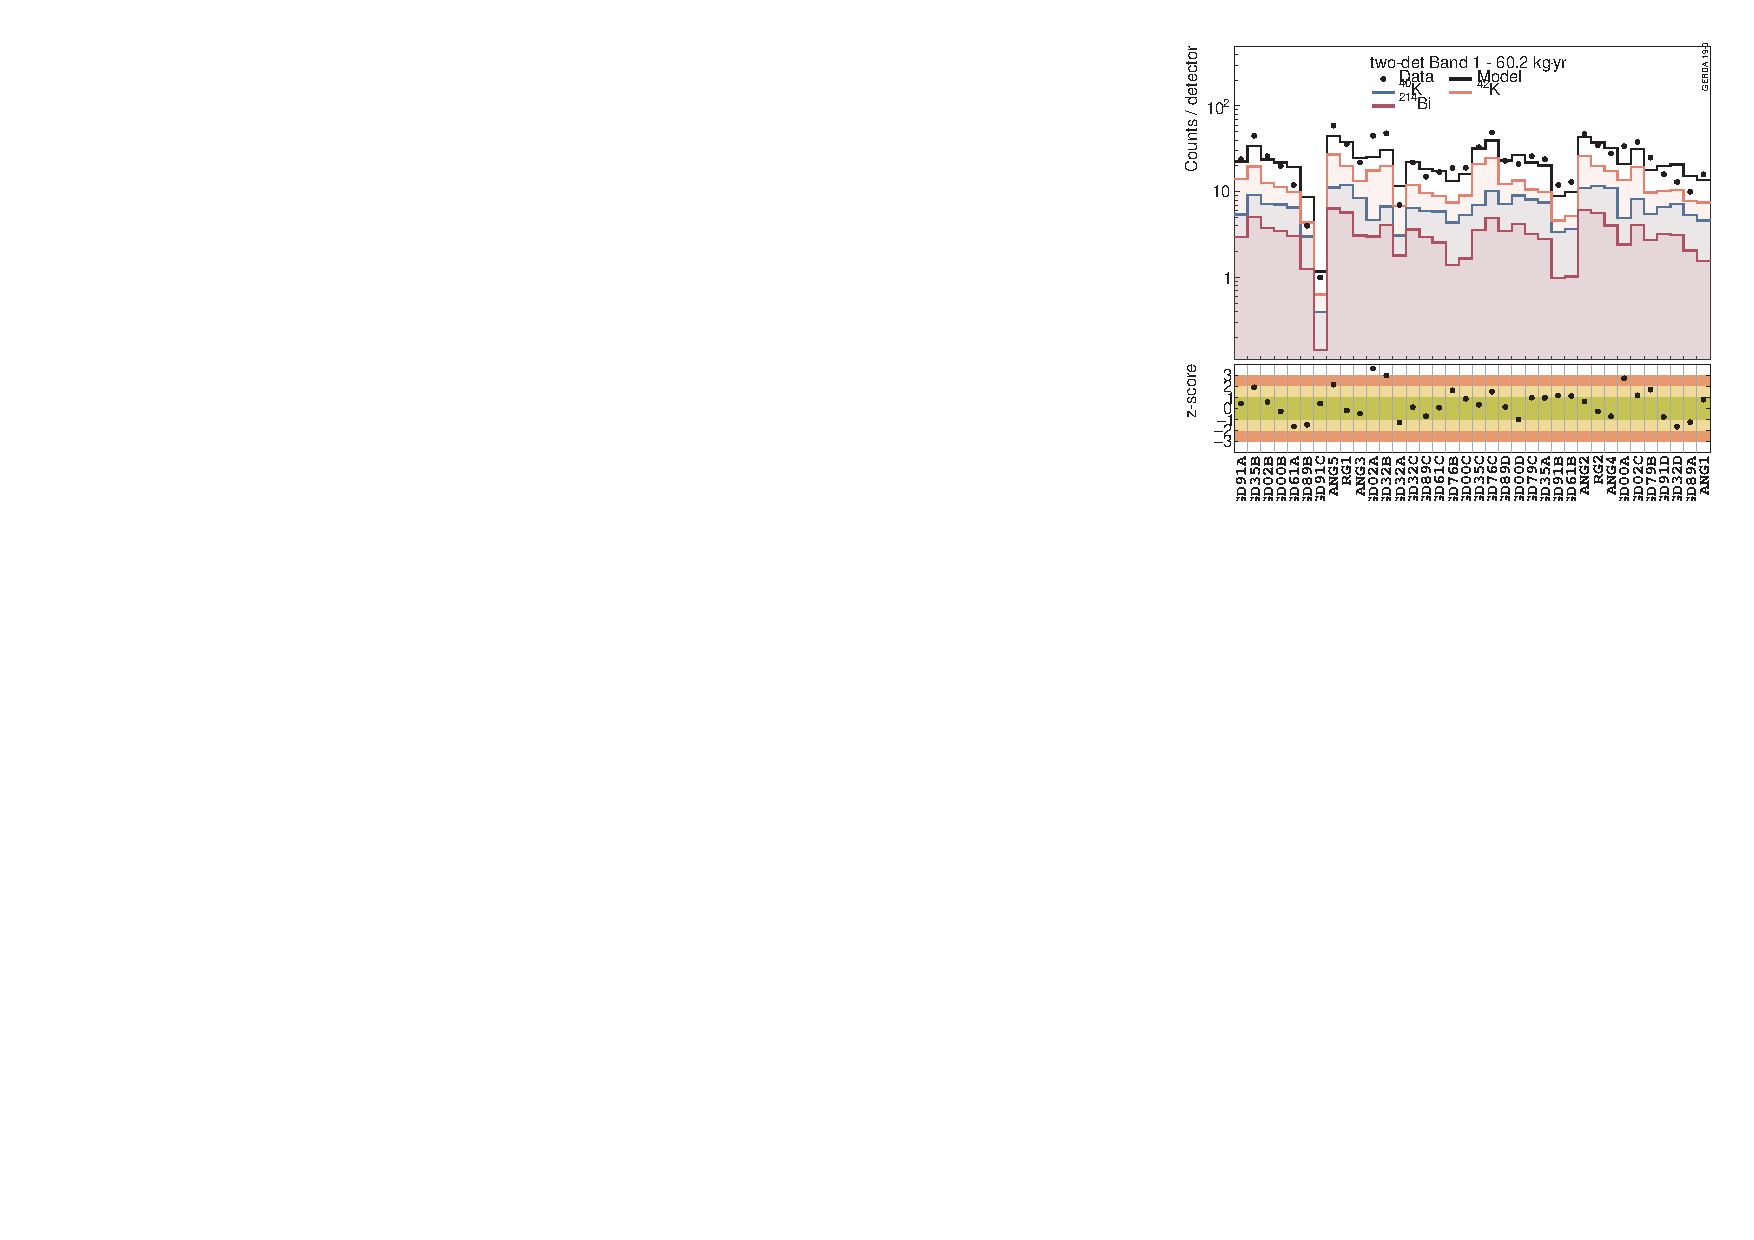
\includegraphics[width=0.45\textwidth]{plots/bkg/raw/ph2/results/kmodel/kmodel-2d-ds7-complete.pdf}
  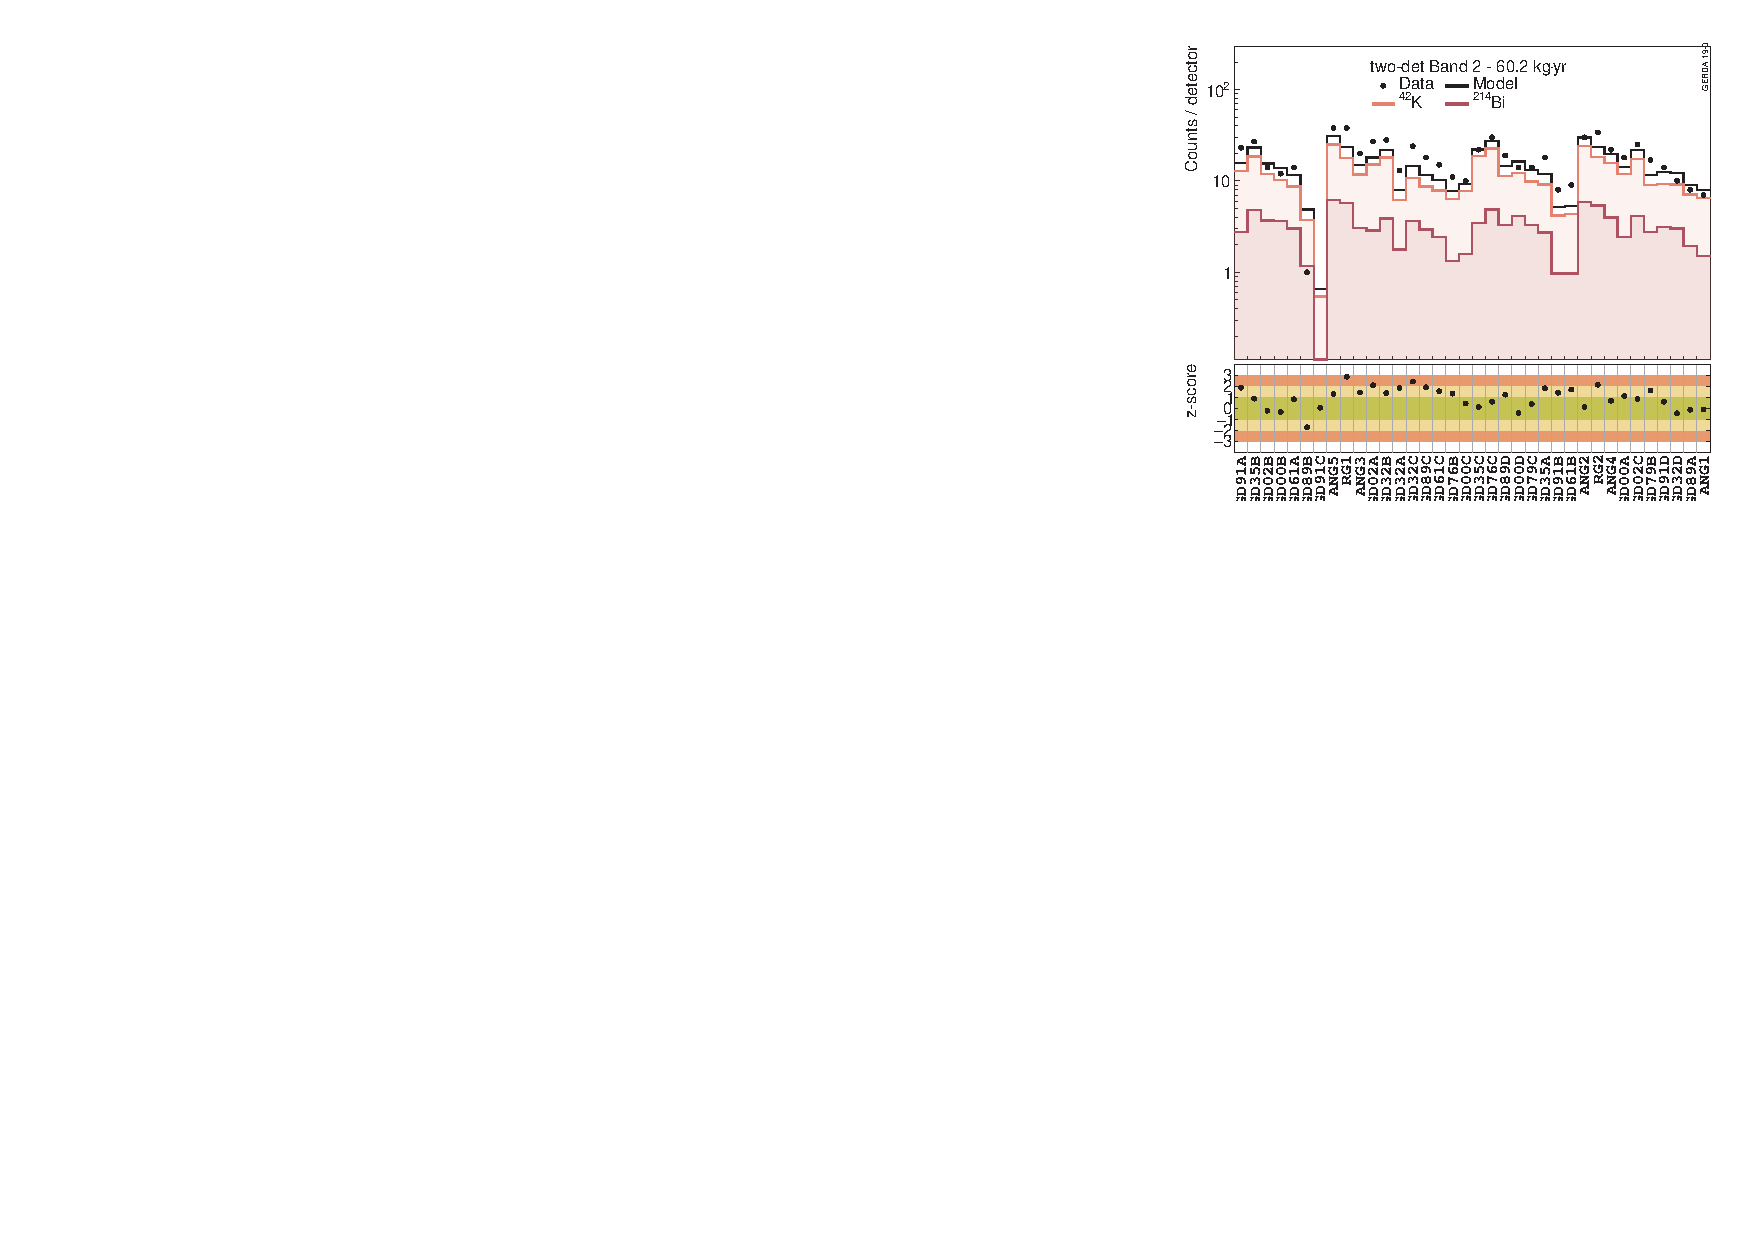
\includegraphics[width=0.45\textwidth]{plots/bkg/raw/ph2/results/kmodel/kmodel-2d-ds8-complete.pdf}\vspace{10pt}
  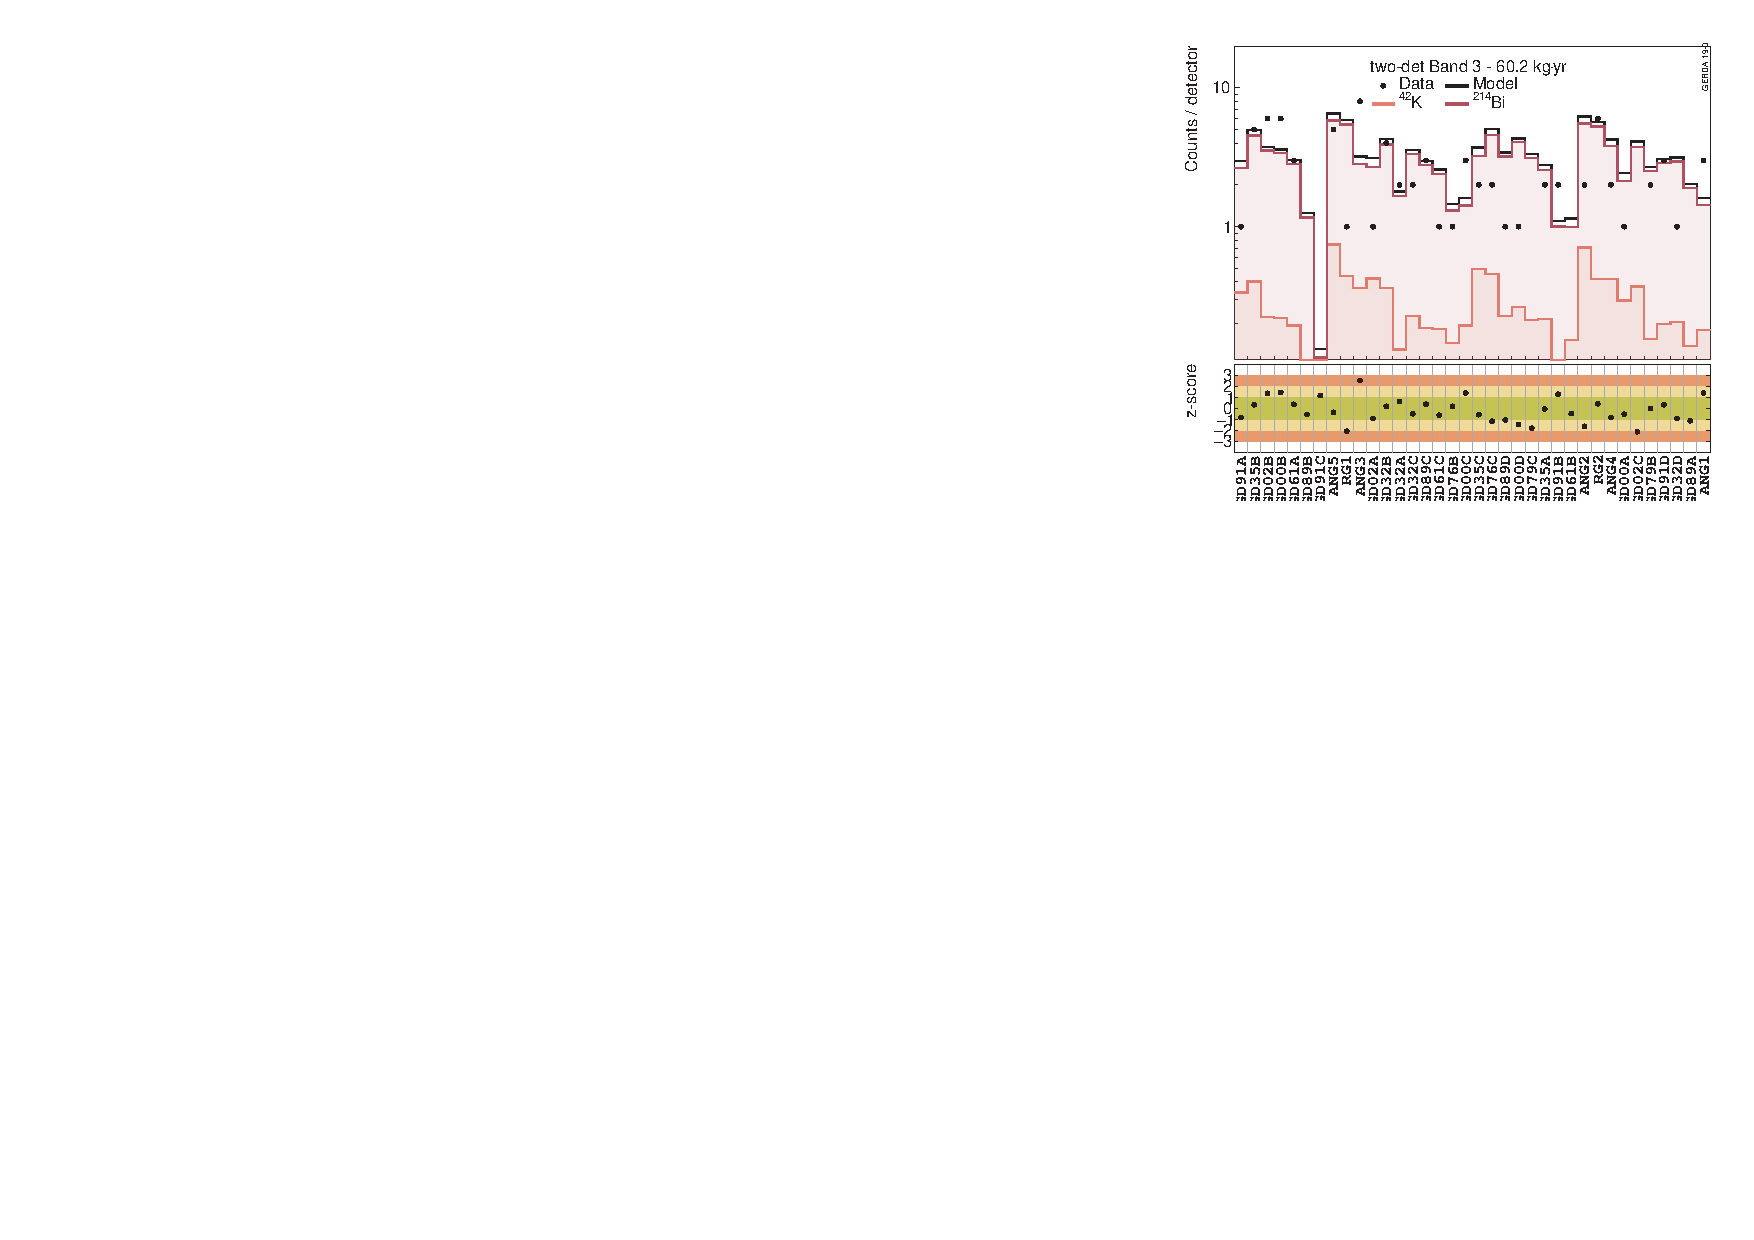
\includegraphics[width=0.45\textwidth]{plots/bkg/raw/ph2/results/kmodel/kmodel-2d-ds9-complete.pdf}
  \begin{minipage}[b][5.3cm][c]{0.45\textwidth}
    \hspace{15pt}%
    \parbox{0.91\textwidth}{%
      \caption{%
        Results of the potassium tracking analysis, two-detector events, extended model (see
        \cref{sec:bkg:raw:ph2:kmodel} for details). To visualize the two-detector data the
        sum of the projections on the two domain axes is shown. Some components are merged
        together to ease the visualization. The \emph{close} and \emph{far} keywords refer
        to the background sources location: close to (cables, holders, mini-shrouds) and far
        from (fibers, SiPMs, copper shrouds, front-end electronics) the detector array.
      }\label{fig:bkg:raw:ph2:kmodel:extended:results:M2}
    }
  \end{minipage}
\end{figure}

% vim: tw=90
